
% Default to the notebook output style

    


% Inherit from the specified cell style.




    
\documentclass[11pt]{article}

    
    
    \usepackage[T1]{fontenc}
    % Nicer default font (+ math font) than Computer Modern for most use cases
    \usepackage{mathpazo}

    % Basic figure setup, for now with no caption control since it's done
    % automatically by Pandoc (which extracts ![](path) syntax from Markdown).
    \usepackage{graphicx}
    % We will generate all images so they have a width \maxwidth. This means
    % that they will get their normal width if they fit onto the page, but
    % are scaled down if they would overflow the margins.
    \makeatletter
    \def\maxwidth{\ifdim\Gin@nat@width>\linewidth\linewidth
    \else\Gin@nat@width\fi}
    \makeatother
    \let\Oldincludegraphics\includegraphics
    % Set max figure width to be 80% of text width, for now hardcoded.
    \renewcommand{\includegraphics}[1]{\Oldincludegraphics[width=.8\maxwidth]{#1}}
    % Ensure that by default, figures have no caption (until we provide a
    % proper Figure object with a Caption API and a way to capture that
    % in the conversion process - todo).
    \usepackage{caption}
    \DeclareCaptionLabelFormat{nolabel}{}
    \captionsetup{labelformat=nolabel}

    \usepackage{adjustbox} % Used to constrain images to a maximum size 
    \usepackage{xcolor} % Allow colors to be defined
    \usepackage{enumerate} % Needed for markdown enumerations to work
    \usepackage{geometry} % Used to adjust the document margins
    \usepackage{amsmath} % Equations
    \usepackage{amssymb} % Equations
    \usepackage{textcomp} % defines textquotesingle
    % Hack from http://tex.stackexchange.com/a/47451/13684:
    \AtBeginDocument{%
        \def\PYZsq{\textquotesingle}% Upright quotes in Pygmentized code
    }
    \usepackage{upquote} % Upright quotes for verbatim code
    \usepackage{eurosym} % defines \euro
    \usepackage[mathletters]{ucs} % Extended unicode (utf-8) support
    \usepackage[utf8x]{inputenc} % Allow utf-8 characters in the tex document
    \usepackage{fancyvrb} % verbatim replacement that allows latex
    \usepackage{grffile} % extends the file name processing of package graphics 
                         % to support a larger range 
    % The hyperref package gives us a pdf with properly built
    % internal navigation ('pdf bookmarks' for the table of contents,
    % internal cross-reference links, web links for URLs, etc.)
    \usepackage{hyperref}
    \usepackage{longtable} % longtable support required by pandoc >1.10
    \usepackage{booktabs}  % table support for pandoc > 1.12.2
    \usepackage[inline]{enumitem} % IRkernel/repr support (it uses the enumerate* environment)
    \usepackage[normalem]{ulem} % ulem is needed to support strikethroughs (\sout)
                                % normalem makes italics be italics, not underlines
    

    
    
    % Colors for the hyperref package
    \definecolor{urlcolor}{rgb}{0,.145,.698}
    \definecolor{linkcolor}{rgb}{.71,0.21,0.01}
    \definecolor{citecolor}{rgb}{.12,.54,.11}

    % ANSI colors
    \definecolor{ansi-black}{HTML}{3E424D}
    \definecolor{ansi-black-intense}{HTML}{282C36}
    \definecolor{ansi-red}{HTML}{E75C58}
    \definecolor{ansi-red-intense}{HTML}{B22B31}
    \definecolor{ansi-green}{HTML}{00A250}
    \definecolor{ansi-green-intense}{HTML}{007427}
    \definecolor{ansi-yellow}{HTML}{DDB62B}
    \definecolor{ansi-yellow-intense}{HTML}{B27D12}
    \definecolor{ansi-blue}{HTML}{208FFB}
    \definecolor{ansi-blue-intense}{HTML}{0065CA}
    \definecolor{ansi-magenta}{HTML}{D160C4}
    \definecolor{ansi-magenta-intense}{HTML}{A03196}
    \definecolor{ansi-cyan}{HTML}{60C6C8}
    \definecolor{ansi-cyan-intense}{HTML}{258F8F}
    \definecolor{ansi-white}{HTML}{C5C1B4}
    \definecolor{ansi-white-intense}{HTML}{A1A6B2}

    % commands and environments needed by pandoc snippets
    % extracted from the output of `pandoc -s`
    \providecommand{\tightlist}{%
      \setlength{\itemsep}{0pt}\setlength{\parskip}{0pt}}
    \DefineVerbatimEnvironment{Highlighting}{Verbatim}{commandchars=\\\{\}}
    % Add ',fontsize=\small' for more characters per line
    \newenvironment{Shaded}{}{}
    \newcommand{\KeywordTok}[1]{\textcolor[rgb]{0.00,0.44,0.13}{\textbf{{#1}}}}
    \newcommand{\DataTypeTok}[1]{\textcolor[rgb]{0.56,0.13,0.00}{{#1}}}
    \newcommand{\DecValTok}[1]{\textcolor[rgb]{0.25,0.63,0.44}{{#1}}}
    \newcommand{\BaseNTok}[1]{\textcolor[rgb]{0.25,0.63,0.44}{{#1}}}
    \newcommand{\FloatTok}[1]{\textcolor[rgb]{0.25,0.63,0.44}{{#1}}}
    \newcommand{\CharTok}[1]{\textcolor[rgb]{0.25,0.44,0.63}{{#1}}}
    \newcommand{\StringTok}[1]{\textcolor[rgb]{0.25,0.44,0.63}{{#1}}}
    \newcommand{\CommentTok}[1]{\textcolor[rgb]{0.38,0.63,0.69}{\textit{{#1}}}}
    \newcommand{\OtherTok}[1]{\textcolor[rgb]{0.00,0.44,0.13}{{#1}}}
    \newcommand{\AlertTok}[1]{\textcolor[rgb]{1.00,0.00,0.00}{\textbf{{#1}}}}
    \newcommand{\FunctionTok}[1]{\textcolor[rgb]{0.02,0.16,0.49}{{#1}}}
    \newcommand{\RegionMarkerTok}[1]{{#1}}
    \newcommand{\ErrorTok}[1]{\textcolor[rgb]{1.00,0.00,0.00}{\textbf{{#1}}}}
    \newcommand{\NormalTok}[1]{{#1}}
    
    % Additional commands for more recent versions of Pandoc
    \newcommand{\ConstantTok}[1]{\textcolor[rgb]{0.53,0.00,0.00}{{#1}}}
    \newcommand{\SpecialCharTok}[1]{\textcolor[rgb]{0.25,0.44,0.63}{{#1}}}
    \newcommand{\VerbatimStringTok}[1]{\textcolor[rgb]{0.25,0.44,0.63}{{#1}}}
    \newcommand{\SpecialStringTok}[1]{\textcolor[rgb]{0.73,0.40,0.53}{{#1}}}
    \newcommand{\ImportTok}[1]{{#1}}
    \newcommand{\DocumentationTok}[1]{\textcolor[rgb]{0.73,0.13,0.13}{\textit{{#1}}}}
    \newcommand{\AnnotationTok}[1]{\textcolor[rgb]{0.38,0.63,0.69}{\textbf{\textit{{#1}}}}}
    \newcommand{\CommentVarTok}[1]{\textcolor[rgb]{0.38,0.63,0.69}{\textbf{\textit{{#1}}}}}
    \newcommand{\VariableTok}[1]{\textcolor[rgb]{0.10,0.09,0.49}{{#1}}}
    \newcommand{\ControlFlowTok}[1]{\textcolor[rgb]{0.00,0.44,0.13}{\textbf{{#1}}}}
    \newcommand{\OperatorTok}[1]{\textcolor[rgb]{0.40,0.40,0.40}{{#1}}}
    \newcommand{\BuiltInTok}[1]{{#1}}
    \newcommand{\ExtensionTok}[1]{{#1}}
    \newcommand{\PreprocessorTok}[1]{\textcolor[rgb]{0.74,0.48,0.00}{{#1}}}
    \newcommand{\AttributeTok}[1]{\textcolor[rgb]{0.49,0.56,0.16}{{#1}}}
    \newcommand{\InformationTok}[1]{\textcolor[rgb]{0.38,0.63,0.69}{\textbf{\textit{{#1}}}}}
    \newcommand{\WarningTok}[1]{\textcolor[rgb]{0.38,0.63,0.69}{\textbf{\textit{{#1}}}}}
    
    
    % Define a nice break command that doesn't care if a line doesn't already
    % exist.
    \def\br{\hspace*{\fill} \\* }
    % Math Jax compatability definitions
    \def\gt{>}
    \def\lt{<}
    % Document parameters
    \title{DIP\_HW9}
    
    
    

    % Pygments definitions
    
\makeatletter
\def\PY@reset{\let\PY@it=\relax \let\PY@bf=\relax%
    \let\PY@ul=\relax \let\PY@tc=\relax%
    \let\PY@bc=\relax \let\PY@ff=\relax}
\def\PY@tok#1{\csname PY@tok@#1\endcsname}
\def\PY@toks#1+{\ifx\relax#1\empty\else%
    \PY@tok{#1}\expandafter\PY@toks\fi}
\def\PY@do#1{\PY@bc{\PY@tc{\PY@ul{%
    \PY@it{\PY@bf{\PY@ff{#1}}}}}}}
\def\PY#1#2{\PY@reset\PY@toks#1+\relax+\PY@do{#2}}

\expandafter\def\csname PY@tok@w\endcsname{\def\PY@tc##1{\textcolor[rgb]{0.73,0.73,0.73}{##1}}}
\expandafter\def\csname PY@tok@c\endcsname{\let\PY@it=\textit\def\PY@tc##1{\textcolor[rgb]{0.25,0.50,0.50}{##1}}}
\expandafter\def\csname PY@tok@cp\endcsname{\def\PY@tc##1{\textcolor[rgb]{0.74,0.48,0.00}{##1}}}
\expandafter\def\csname PY@tok@k\endcsname{\let\PY@bf=\textbf\def\PY@tc##1{\textcolor[rgb]{0.00,0.50,0.00}{##1}}}
\expandafter\def\csname PY@tok@kp\endcsname{\def\PY@tc##1{\textcolor[rgb]{0.00,0.50,0.00}{##1}}}
\expandafter\def\csname PY@tok@kt\endcsname{\def\PY@tc##1{\textcolor[rgb]{0.69,0.00,0.25}{##1}}}
\expandafter\def\csname PY@tok@o\endcsname{\def\PY@tc##1{\textcolor[rgb]{0.40,0.40,0.40}{##1}}}
\expandafter\def\csname PY@tok@ow\endcsname{\let\PY@bf=\textbf\def\PY@tc##1{\textcolor[rgb]{0.67,0.13,1.00}{##1}}}
\expandafter\def\csname PY@tok@nb\endcsname{\def\PY@tc##1{\textcolor[rgb]{0.00,0.50,0.00}{##1}}}
\expandafter\def\csname PY@tok@nf\endcsname{\def\PY@tc##1{\textcolor[rgb]{0.00,0.00,1.00}{##1}}}
\expandafter\def\csname PY@tok@nc\endcsname{\let\PY@bf=\textbf\def\PY@tc##1{\textcolor[rgb]{0.00,0.00,1.00}{##1}}}
\expandafter\def\csname PY@tok@nn\endcsname{\let\PY@bf=\textbf\def\PY@tc##1{\textcolor[rgb]{0.00,0.00,1.00}{##1}}}
\expandafter\def\csname PY@tok@ne\endcsname{\let\PY@bf=\textbf\def\PY@tc##1{\textcolor[rgb]{0.82,0.25,0.23}{##1}}}
\expandafter\def\csname PY@tok@nv\endcsname{\def\PY@tc##1{\textcolor[rgb]{0.10,0.09,0.49}{##1}}}
\expandafter\def\csname PY@tok@no\endcsname{\def\PY@tc##1{\textcolor[rgb]{0.53,0.00,0.00}{##1}}}
\expandafter\def\csname PY@tok@nl\endcsname{\def\PY@tc##1{\textcolor[rgb]{0.63,0.63,0.00}{##1}}}
\expandafter\def\csname PY@tok@ni\endcsname{\let\PY@bf=\textbf\def\PY@tc##1{\textcolor[rgb]{0.60,0.60,0.60}{##1}}}
\expandafter\def\csname PY@tok@na\endcsname{\def\PY@tc##1{\textcolor[rgb]{0.49,0.56,0.16}{##1}}}
\expandafter\def\csname PY@tok@nt\endcsname{\let\PY@bf=\textbf\def\PY@tc##1{\textcolor[rgb]{0.00,0.50,0.00}{##1}}}
\expandafter\def\csname PY@tok@nd\endcsname{\def\PY@tc##1{\textcolor[rgb]{0.67,0.13,1.00}{##1}}}
\expandafter\def\csname PY@tok@s\endcsname{\def\PY@tc##1{\textcolor[rgb]{0.73,0.13,0.13}{##1}}}
\expandafter\def\csname PY@tok@sd\endcsname{\let\PY@it=\textit\def\PY@tc##1{\textcolor[rgb]{0.73,0.13,0.13}{##1}}}
\expandafter\def\csname PY@tok@si\endcsname{\let\PY@bf=\textbf\def\PY@tc##1{\textcolor[rgb]{0.73,0.40,0.53}{##1}}}
\expandafter\def\csname PY@tok@se\endcsname{\let\PY@bf=\textbf\def\PY@tc##1{\textcolor[rgb]{0.73,0.40,0.13}{##1}}}
\expandafter\def\csname PY@tok@sr\endcsname{\def\PY@tc##1{\textcolor[rgb]{0.73,0.40,0.53}{##1}}}
\expandafter\def\csname PY@tok@ss\endcsname{\def\PY@tc##1{\textcolor[rgb]{0.10,0.09,0.49}{##1}}}
\expandafter\def\csname PY@tok@sx\endcsname{\def\PY@tc##1{\textcolor[rgb]{0.00,0.50,0.00}{##1}}}
\expandafter\def\csname PY@tok@m\endcsname{\def\PY@tc##1{\textcolor[rgb]{0.40,0.40,0.40}{##1}}}
\expandafter\def\csname PY@tok@gh\endcsname{\let\PY@bf=\textbf\def\PY@tc##1{\textcolor[rgb]{0.00,0.00,0.50}{##1}}}
\expandafter\def\csname PY@tok@gu\endcsname{\let\PY@bf=\textbf\def\PY@tc##1{\textcolor[rgb]{0.50,0.00,0.50}{##1}}}
\expandafter\def\csname PY@tok@gd\endcsname{\def\PY@tc##1{\textcolor[rgb]{0.63,0.00,0.00}{##1}}}
\expandafter\def\csname PY@tok@gi\endcsname{\def\PY@tc##1{\textcolor[rgb]{0.00,0.63,0.00}{##1}}}
\expandafter\def\csname PY@tok@gr\endcsname{\def\PY@tc##1{\textcolor[rgb]{1.00,0.00,0.00}{##1}}}
\expandafter\def\csname PY@tok@ge\endcsname{\let\PY@it=\textit}
\expandafter\def\csname PY@tok@gs\endcsname{\let\PY@bf=\textbf}
\expandafter\def\csname PY@tok@gp\endcsname{\let\PY@bf=\textbf\def\PY@tc##1{\textcolor[rgb]{0.00,0.00,0.50}{##1}}}
\expandafter\def\csname PY@tok@go\endcsname{\def\PY@tc##1{\textcolor[rgb]{0.53,0.53,0.53}{##1}}}
\expandafter\def\csname PY@tok@gt\endcsname{\def\PY@tc##1{\textcolor[rgb]{0.00,0.27,0.87}{##1}}}
\expandafter\def\csname PY@tok@err\endcsname{\def\PY@bc##1{\setlength{\fboxsep}{0pt}\fcolorbox[rgb]{1.00,0.00,0.00}{1,1,1}{\strut ##1}}}
\expandafter\def\csname PY@tok@kc\endcsname{\let\PY@bf=\textbf\def\PY@tc##1{\textcolor[rgb]{0.00,0.50,0.00}{##1}}}
\expandafter\def\csname PY@tok@kd\endcsname{\let\PY@bf=\textbf\def\PY@tc##1{\textcolor[rgb]{0.00,0.50,0.00}{##1}}}
\expandafter\def\csname PY@tok@kn\endcsname{\let\PY@bf=\textbf\def\PY@tc##1{\textcolor[rgb]{0.00,0.50,0.00}{##1}}}
\expandafter\def\csname PY@tok@kr\endcsname{\let\PY@bf=\textbf\def\PY@tc##1{\textcolor[rgb]{0.00,0.50,0.00}{##1}}}
\expandafter\def\csname PY@tok@bp\endcsname{\def\PY@tc##1{\textcolor[rgb]{0.00,0.50,0.00}{##1}}}
\expandafter\def\csname PY@tok@fm\endcsname{\def\PY@tc##1{\textcolor[rgb]{0.00,0.00,1.00}{##1}}}
\expandafter\def\csname PY@tok@vc\endcsname{\def\PY@tc##1{\textcolor[rgb]{0.10,0.09,0.49}{##1}}}
\expandafter\def\csname PY@tok@vg\endcsname{\def\PY@tc##1{\textcolor[rgb]{0.10,0.09,0.49}{##1}}}
\expandafter\def\csname PY@tok@vi\endcsname{\def\PY@tc##1{\textcolor[rgb]{0.10,0.09,0.49}{##1}}}
\expandafter\def\csname PY@tok@vm\endcsname{\def\PY@tc##1{\textcolor[rgb]{0.10,0.09,0.49}{##1}}}
\expandafter\def\csname PY@tok@sa\endcsname{\def\PY@tc##1{\textcolor[rgb]{0.73,0.13,0.13}{##1}}}
\expandafter\def\csname PY@tok@sb\endcsname{\def\PY@tc##1{\textcolor[rgb]{0.73,0.13,0.13}{##1}}}
\expandafter\def\csname PY@tok@sc\endcsname{\def\PY@tc##1{\textcolor[rgb]{0.73,0.13,0.13}{##1}}}
\expandafter\def\csname PY@tok@dl\endcsname{\def\PY@tc##1{\textcolor[rgb]{0.73,0.13,0.13}{##1}}}
\expandafter\def\csname PY@tok@s2\endcsname{\def\PY@tc##1{\textcolor[rgb]{0.73,0.13,0.13}{##1}}}
\expandafter\def\csname PY@tok@sh\endcsname{\def\PY@tc##1{\textcolor[rgb]{0.73,0.13,0.13}{##1}}}
\expandafter\def\csname PY@tok@s1\endcsname{\def\PY@tc##1{\textcolor[rgb]{0.73,0.13,0.13}{##1}}}
\expandafter\def\csname PY@tok@mb\endcsname{\def\PY@tc##1{\textcolor[rgb]{0.40,0.40,0.40}{##1}}}
\expandafter\def\csname PY@tok@mf\endcsname{\def\PY@tc##1{\textcolor[rgb]{0.40,0.40,0.40}{##1}}}
\expandafter\def\csname PY@tok@mh\endcsname{\def\PY@tc##1{\textcolor[rgb]{0.40,0.40,0.40}{##1}}}
\expandafter\def\csname PY@tok@mi\endcsname{\def\PY@tc##1{\textcolor[rgb]{0.40,0.40,0.40}{##1}}}
\expandafter\def\csname PY@tok@il\endcsname{\def\PY@tc##1{\textcolor[rgb]{0.40,0.40,0.40}{##1}}}
\expandafter\def\csname PY@tok@mo\endcsname{\def\PY@tc##1{\textcolor[rgb]{0.40,0.40,0.40}{##1}}}
\expandafter\def\csname PY@tok@ch\endcsname{\let\PY@it=\textit\def\PY@tc##1{\textcolor[rgb]{0.25,0.50,0.50}{##1}}}
\expandafter\def\csname PY@tok@cm\endcsname{\let\PY@it=\textit\def\PY@tc##1{\textcolor[rgb]{0.25,0.50,0.50}{##1}}}
\expandafter\def\csname PY@tok@cpf\endcsname{\let\PY@it=\textit\def\PY@tc##1{\textcolor[rgb]{0.25,0.50,0.50}{##1}}}
\expandafter\def\csname PY@tok@c1\endcsname{\let\PY@it=\textit\def\PY@tc##1{\textcolor[rgb]{0.25,0.50,0.50}{##1}}}
\expandafter\def\csname PY@tok@cs\endcsname{\let\PY@it=\textit\def\PY@tc##1{\textcolor[rgb]{0.25,0.50,0.50}{##1}}}

\def\PYZbs{\char`\\}
\def\PYZus{\char`\_}
\def\PYZob{\char`\{}
\def\PYZcb{\char`\}}
\def\PYZca{\char`\^}
\def\PYZam{\char`\&}
\def\PYZlt{\char`\<}
\def\PYZgt{\char`\>}
\def\PYZsh{\char`\#}
\def\PYZpc{\char`\%}
\def\PYZdl{\char`\$}
\def\PYZhy{\char`\-}
\def\PYZsq{\char`\'}
\def\PYZdq{\char`\"}
\def\PYZti{\char`\~}
% for compatibility with earlier versions
\def\PYZat{@}
\def\PYZlb{[}
\def\PYZrb{]}
\makeatother


    % Exact colors from NB
    \definecolor{incolor}{rgb}{0.0, 0.0, 0.5}
    \definecolor{outcolor}{rgb}{0.545, 0.0, 0.0}



    
    % Prevent overflowing lines due to hard-to-break entities
    \sloppy 
    % Setup hyperref package
    \hypersetup{
      breaklinks=true,  % so long urls are correctly broken across lines
      colorlinks=true,
      urlcolor=urlcolor,
      linkcolor=linkcolor,
      citecolor=citecolor,
      }
    % Slightly bigger margins than the latex defaults
    
    \geometry{verbose,tmargin=1in,bmargin=1in,lmargin=1in,rmargin=1in}
    
    

    \begin{document}
    
    
    \maketitle
    
    

    
    \hypertarget{digital-image-processing---hw9---98722278---mohammad-doosti-lakhani}{%
\section{Digital Image Processing - HW9 - 98722278 - Mohammad Doosti
Lakhani}\label{digital-image-processing---hw9---98722278---mohammad-doosti-lakhani}}

In this notebook, I have solved the assignment's problems which are as
follows:

\begin{enumerate}
\def\labelenumi{\arabic{enumi}.}
\tightlist
\item
  Consider this image and determine the type of morphological operation
  and structural element by defining its center:
\end{enumerate}

\begin{figure}
\centering

\includegraphics{wiki/1_1.jpg}
\caption{q1 im1}
\end{figure}

A. 
\includegraphics{wiki/1_2.jpg} B. 
\includegraphics{wiki/1_3.jpg} C.

\includegraphics{wiki/1_4.jpg} D. 
\includegraphics{wiki/1_5.jpg}

\begin{enumerate}
\def\labelenumi{\arabic{enumi}.}
\setcounter{enumi}{1}
\tightlist
\item
  Given the sets as below images, draw the result of the given
  morphological operations:
\end{enumerate}

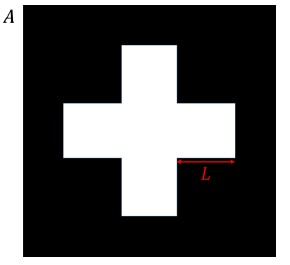
\includegraphics{wiki/2_1.jpg} 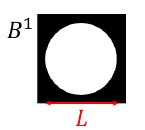
\includegraphics{wiki/2_2.jpg}
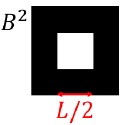
\includegraphics{wiki/2_3.jpg} 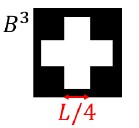
\includegraphics{wiki/2_4.jpg}
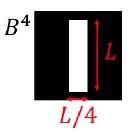
\includegraphics{wiki/2_5.jpg}

\begin{verbatim}
1. (A ⊝ B4) ⊕ B2
2. (A ⊝ B1) ⊕ B3
3. (A ⊕ B4) ⊕ B2
4. (A ⊕ B2) ⊝ B3
\end{verbatim}

\begin{enumerate}
\def\labelenumi{\arabic{enumi}.}
\setcounter{enumi}{2}
\tightlist
\item
  Do this tasks for this question:

  \begin{enumerate}
  \def\labelenumii{\arabic{enumii}.}
  \tightlist
  \item
    \textbf{Hit-or-Miss} operation has been explained in section 9.4 in
    the book (Gonsalez), explain it.
  \item
    Read this
    \href{http://www.ee.oulu.fi/research/mvmp/mvg/files/pdf/ahonen_soft_histograms_for_local_binary_patterns.pdf}{paper}
    and compare \textbf{LBP} and \textbf{Soft LBP}.
  \end{enumerate}
\item
  Train and evalute a model for Farsi handwritten digit recognition

  \begin{enumerate}
  \def\labelenumii{\arabic{enumii}.}
  \tightlist
  \item
    Use this dataset https://github.com/amir-saniyan/HodaDatasetReader
  \item
    Use Feature extraction such a texture
  \item
    Use \textbf{SVM} and \textbf{kNN} for learning process as mandatory
    classifiers
  \item
    Other classifiers (optional)
  \item
    Evalute model using confustion matrix and average accuracy
  \item
    Compare results w.r.t. different features (optional)
  \end{enumerate}
\end{enumerate}

    \hypertarget{consider-this-image-and-determine-the-type-of-morphological-operation-and-structural-element-by-defining-its-center}{%
\subsection{1 Consider this image and determine the type of
morphological operation and structural element by defining its
center:}\label{consider-this-image-and-determine-the-type-of-morphological-operation-and-structural-element-by-defining-its-center}}

\begin{figure}
\centering

\includegraphics{wiki/1_1.jpg}
\caption{q1 im1}
\end{figure}

\begin{enumerate}
\def\labelenumi{\arabic{enumi}.}
\tightlist
\item
  
\includegraphics{wiki/1_2.jpg} 2. 
\includegraphics{wiki/1_3.jpg} 3.
  
\includegraphics{wiki/1_4.jpg} 4. 
\includegraphics{wiki/1_5.jpg}
\end{enumerate}

    \begin{figure}
\centering
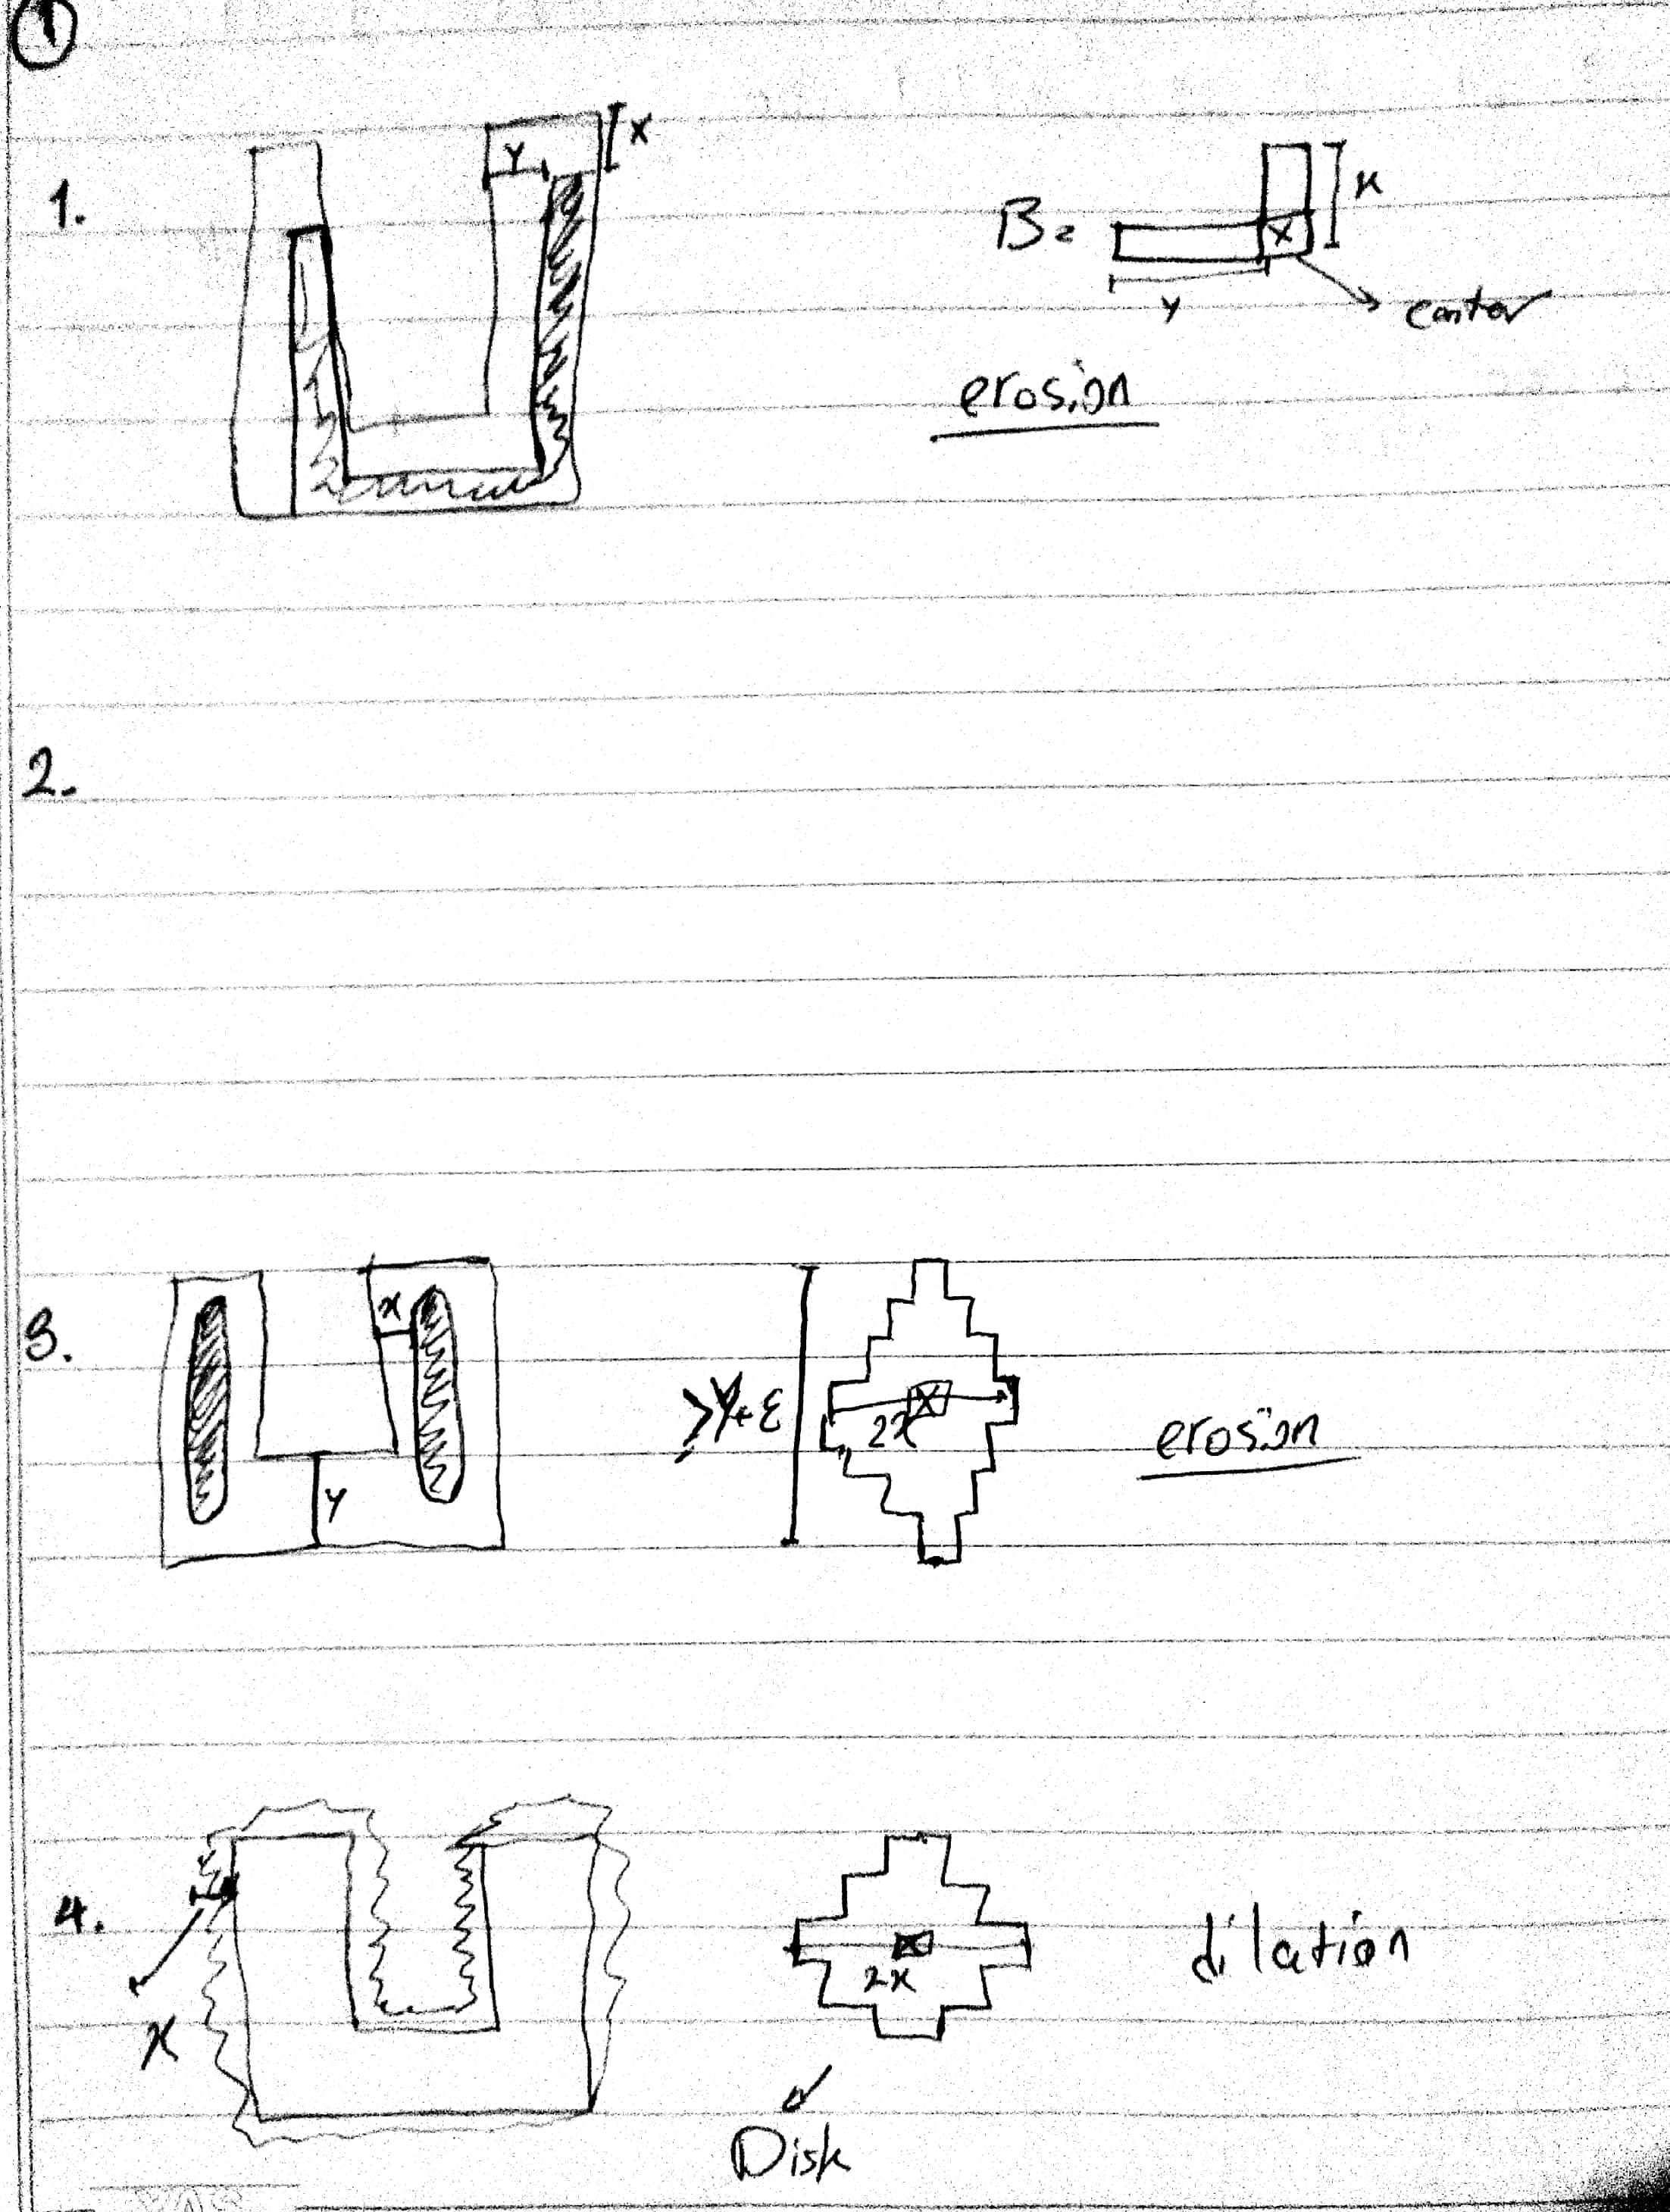
\includegraphics{wiki/1_6.jpg}
\caption{answer of question 1}
\end{figure}

    \hypertarget{given-the-sets-as-below-images-draw-the-result-of-the-given-morphological-operations}{%
\subsection{2 Given the sets as below images, draw the result of the
given morphological
operations:}\label{given-the-sets-as-below-images-draw-the-result-of-the-given-morphological-operations}}

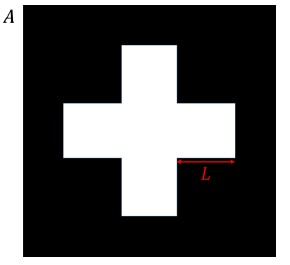
\includegraphics{wiki/2_1.jpg} 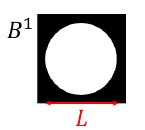
\includegraphics{wiki/2_2.jpg}
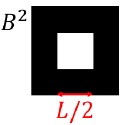
\includegraphics{wiki/2_3.jpg} 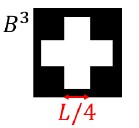
\includegraphics{wiki/2_4.jpg}
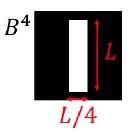
\includegraphics{wiki/2_5.jpg}

\begin{enumerate}
\def\labelenumi{\arabic{enumi}.}
\tightlist
\item
  (A ⊝ B4) ⊕ B2
\item
  (A ⊝ B1) ⊕ B3
\item
  (A ⊕ B4) ⊕ B2
\item
  (A ⊕ B2) ⊝ B3
\end{enumerate}

    \begin{figure}
\centering
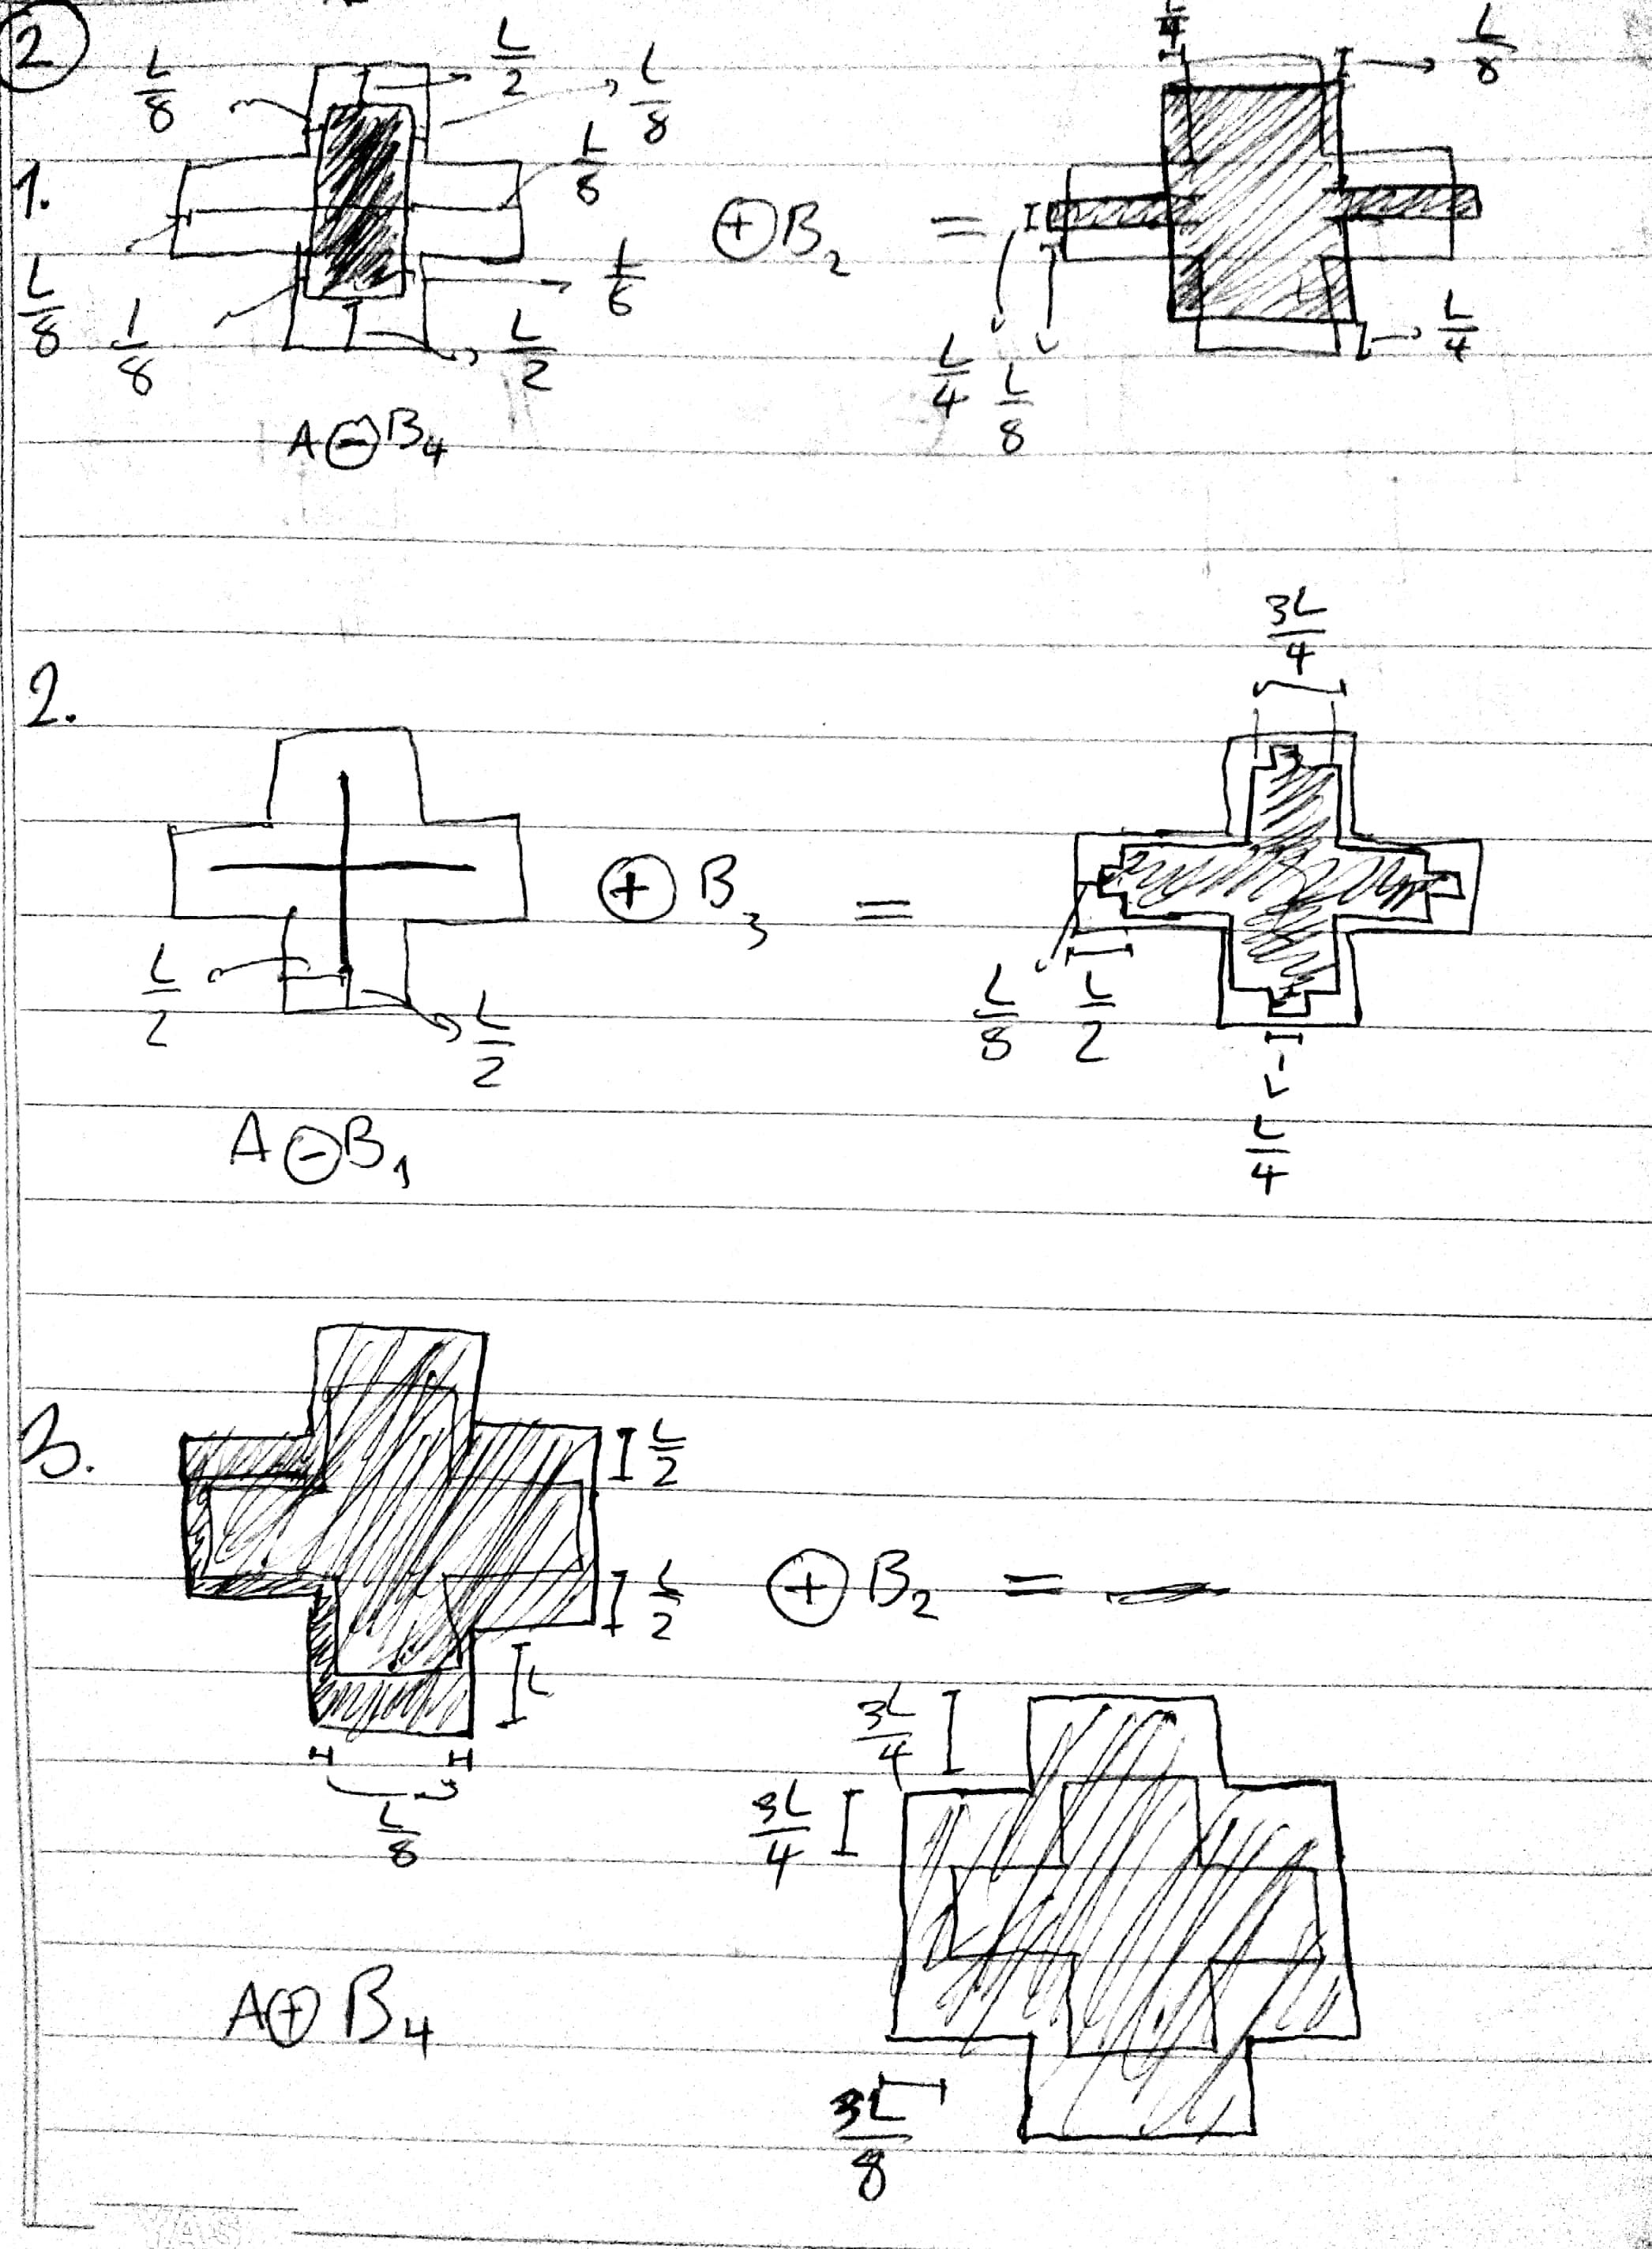
\includegraphics{wiki/2_6.jpg}
\caption{answer1 to question 2}
\end{figure}

\begin{figure}
\centering
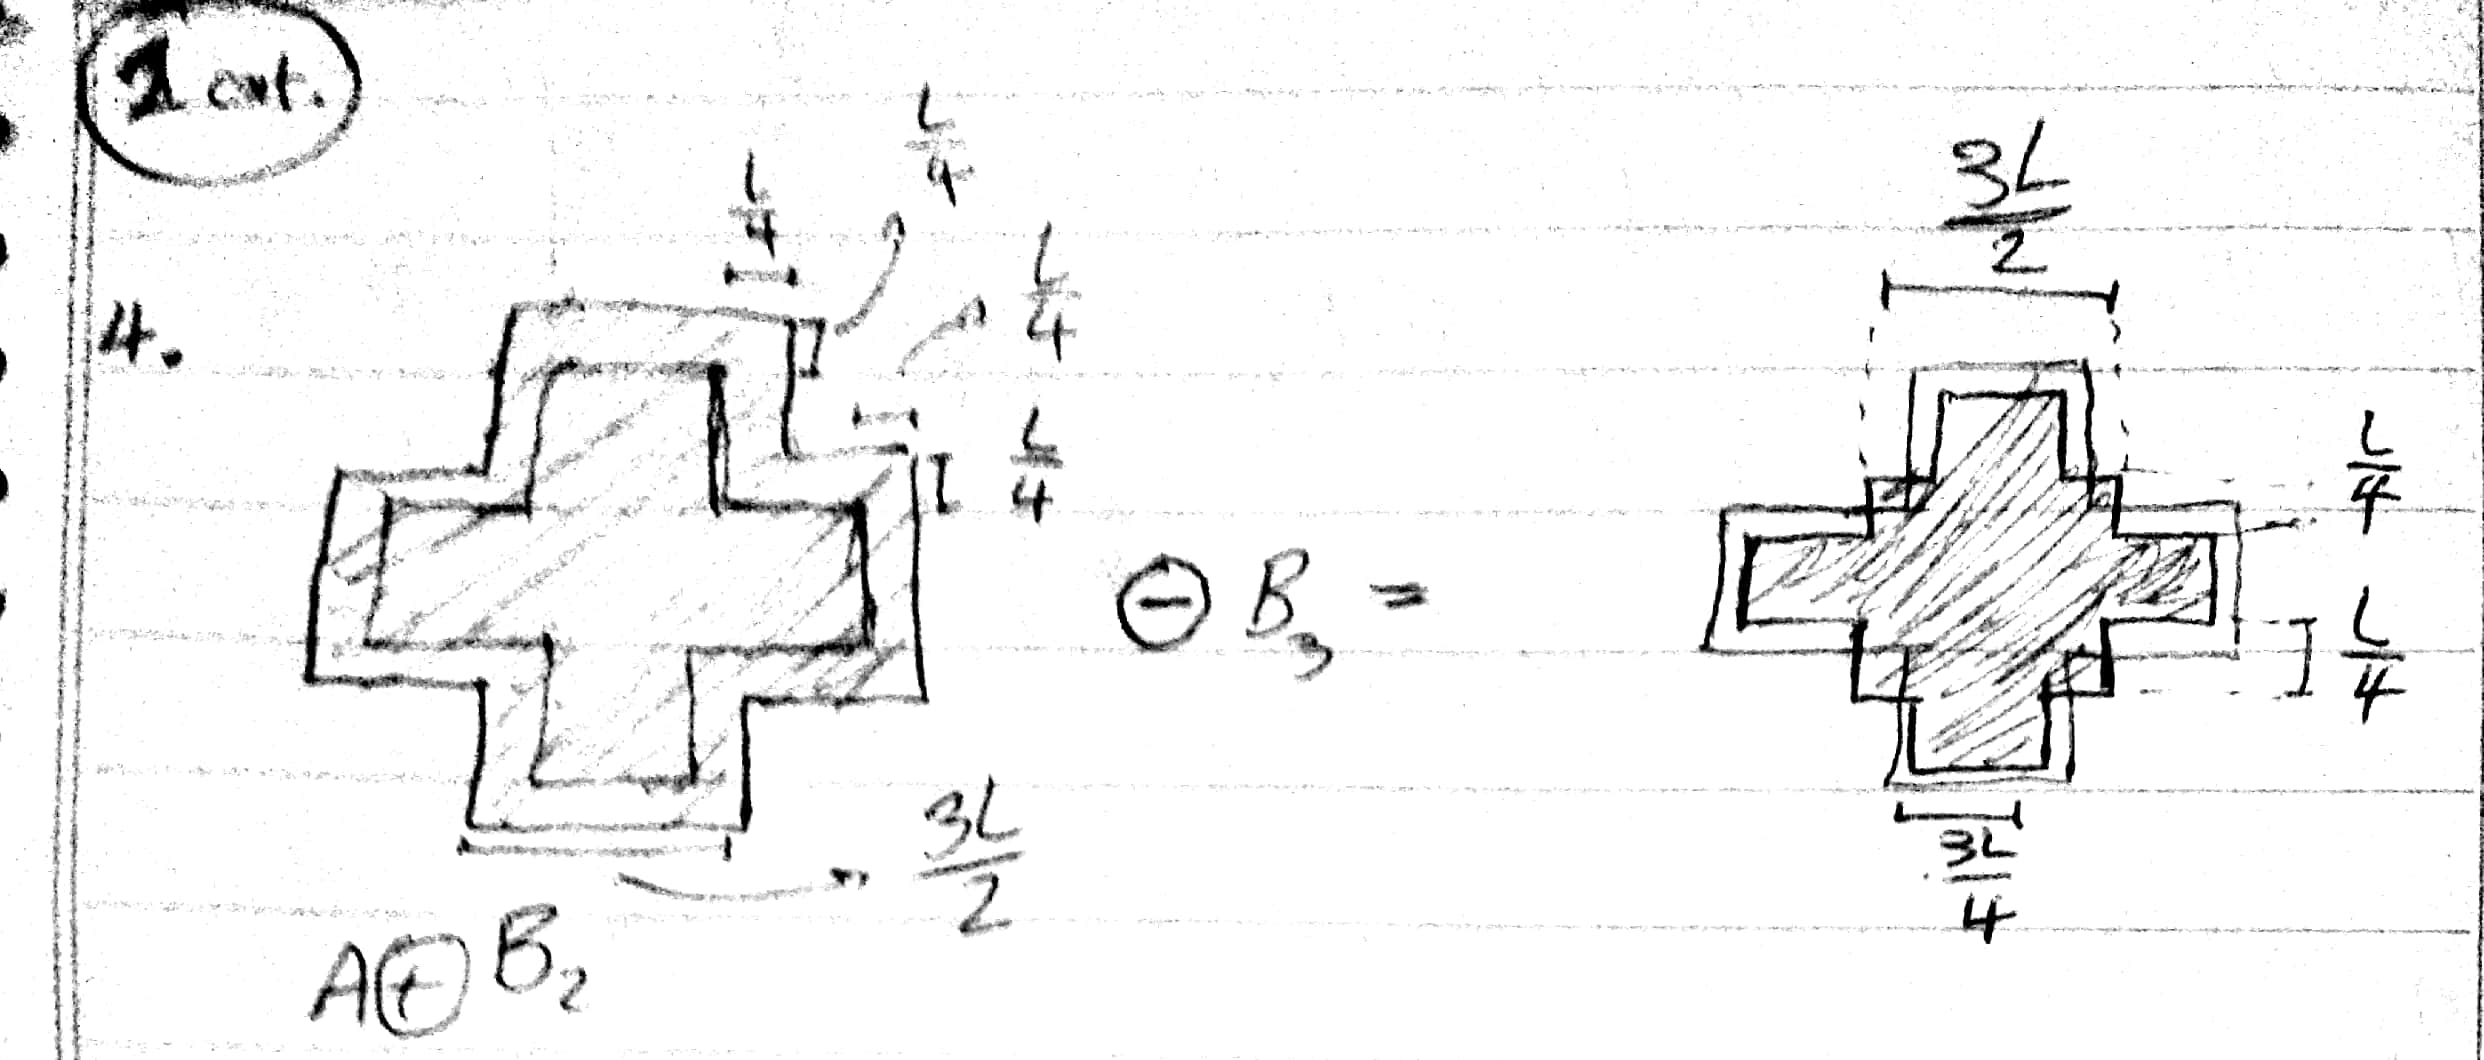
\includegraphics{wiki/2_7.jpg}
\caption{answer2 to question 2}
\end{figure}

    \hypertarget{do-this-tasks-for-this-question}{%
\subsection{3 Do this tasks for this
question:}\label{do-this-tasks-for-this-question}}

\begin{enumerate}
\def\labelenumi{\arabic{enumi}.}
\tightlist
\item
  \textbf{Hit-or-Miss} operation has been explained in section 9.4 in
  the book (Gonzales), explain it.
\item
  Read this
  \href{http://www.ee.oulu.fi/research/mvmp/mvg/files/pdf/ahonen_soft_histograms_for_local_binary_patterns.pdf}{paper}
  and compare \textbf{LBP} and \textbf{Soft LBP}.
\end{enumerate}

    \hypertarget{a-hit-or-miss-operator}{%
\subsubsection{\texorpdfstring{3. A \textbf{Hit-or-Miss}
Operator}{3. A Hit-or-Miss Operator}}\label{a-hit-or-miss-operator}}

First thing we need to know is that HOM is used for basic shape
detection which works on binary images where 1s indicate foreground and
0s for background.

HOM uses two structural elements, one for foreground and one for
background.

Here is the matchematical definition of it:

\begin{figure}
\centering
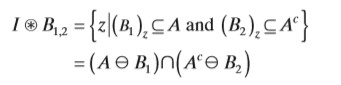
\includegraphics{wiki/3_1_1.jpg}
\caption{HOM formula}
\end{figure}

Intuitively, it says that foreground and background structural elements
must match simultaneously. But we also can represent same operation
using only one structural element, here is the matchematical definition:

\begin{figure}
\centering

\includegraphics{wiki/3_1_2.jpg}
\caption{HOM formula 2}
\end{figure}

In this situation, structural element \textbf{B} consisits of both
foreground and background pixels and that is why we need to do the
operation simultaneously. In simple words, in erosion we just check for
foreground elements but in this operation, we match foreground pixels of
structural element with foreground pixels of image and \textbf{at the
same time} wew also match background pixels of structural element with
background pixels of image.

As a simple example, let's say we want to find a dot in image. We need
that it means that a single foreground pixel should be surrended by many
background pixels in all directions. So same structural element will be
used and only would match when a single foreground pixel get surrended
by background pixels.

Here is 3 examples of this operation:

\begin{figure}
\centering
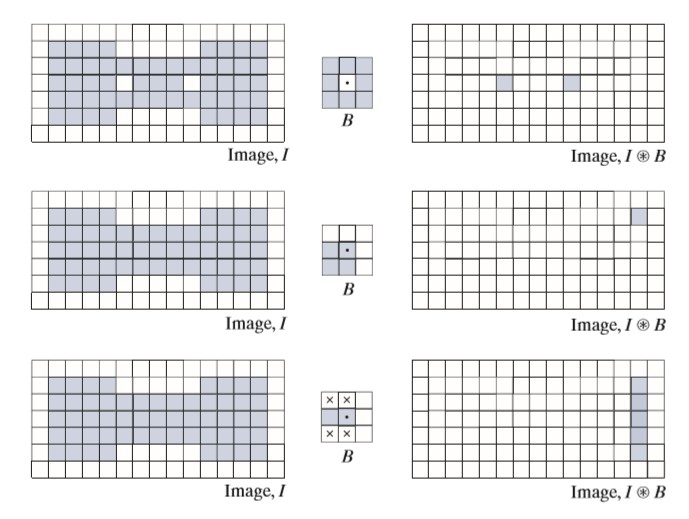
\includegraphics{wiki/3_1_3.jpg}
\caption{HOM examples}
\end{figure}

    \hypertarget{b-compare-soft-lbp-and-lbp}{%
\subsubsection{3.B Compare Soft LBP and
LBP}\label{b-compare-soft-lbp-and-lbp}}

Soft LBP's major charactrestic is rebustness against noises and
continuous output w.r.t. inputs which also can work well on degraded
images.

So let's first talk about LBP itself and what makes it special. It is
fast and invariant to gray-scale intensity changes which makes it
tolerant against illumination changes which can be used for texture
classification, face analysis, etc.

The possible problem of basic LBP could be the fixed thresholding
regarding neighboring pixels where could make it very sensitive to
noises.

Basic LBP compare pixels in a 3x3 window and mark lower ones zero and
vice versa. Finally, summing up by weighting to power of 2 would be our
desired output. This operation and its thresholding window can be
represented using below depictions where P is number of sampling points
on a circle of radius of R:

\begin{figure}
\centering
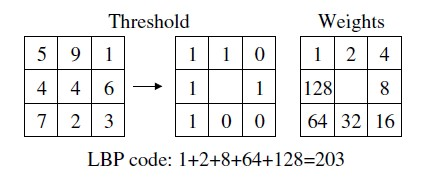
\includegraphics{wiki/3_2_1.jpg}
\caption{fixed thresold}
\end{figure}

\begin{figure}
\centering
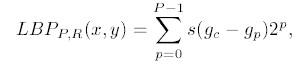
\includegraphics{wiki/3_2_2.jpg}
\caption{basic LBP}
\end{figure}

Where the problem is the thresholding function which is as follow:

\begin{figure}
\centering
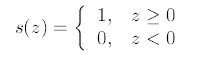
\includegraphics{wiki/3_2_3.jpg}
\caption{basic LBP Thresholding}
\end{figure}

So as we knew it from the begining the goal is to increase robustness
via fuzzy membership function and here is the new defined functions
where the parameter D controls the amount of fuzzification:

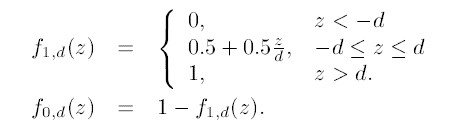
\includegraphics{wiki/3_2_4.jpg} 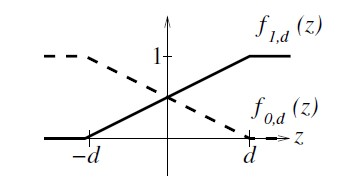
\includegraphics{wiki/3_2_6.jpg}

To build the histogram, now each pixel instead of contributing to only
one bin where happens in basic LBP, now contributes to all bins
regarding the membership function where sums up to 1 over all bins:

\begin{figure}
\centering
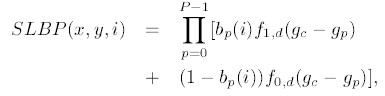
\includegraphics{wiki/3_2_5.jpg}
\caption{pixel in bin of histogram in soft LBP}
\end{figure}

By using this membership functions, soft LBP looses one of the upsides
of the basic LBP which is invariance to gray-level illumination. But the
upside effect is that small changes introduces small effects too. On top
of that, another issue affecting Soft LBP is that this method is
computationally expensive because the contribution of the each pixel
need to be computed w.r.t. all 2\^{}P bins.

These result comparsion could be great to finish explanation.

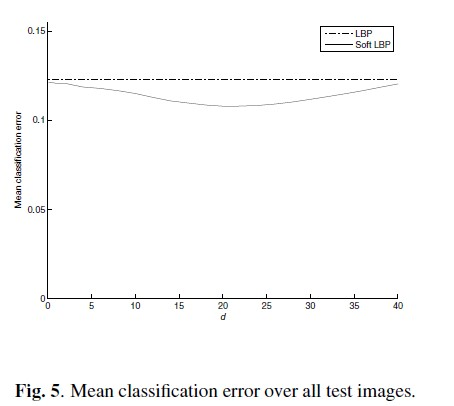
\includegraphics{wiki/3_2_7.jpg} 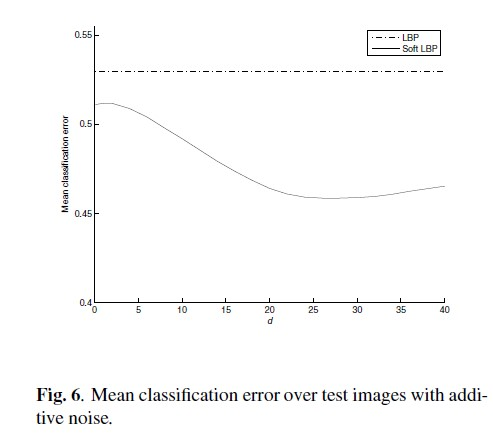
\includegraphics{wiki/3_2_8.jpg}

    \hypertarget{train-and-evalute-a-model-for-farsi-handwritten-digit-recognition}{%
\subsection{4 Train and evalute a model for Farsi handwritten digit
recognition}\label{train-and-evalute-a-model-for-farsi-handwritten-digit-recognition}}

\begin{enumerate}
\def\labelenumi{\arabic{enumi}.}
\tightlist
\item
  Use this dataset https://github.com/amir-saniyan/HodaDatasetReader
\item
  Use Features such a texture and geometry
\item
  Use \textbf{SVM} and \textbf{kNN} for learning process as mandatory
  classifiers
\item
  Evalute model using confustion matrix and average accuracy
\item
  Compare results w.r.t. different features (optional)
\end{enumerate}

    \begin{Verbatim}[commandchars=\\\{\}]
{\color{incolor}In [{\color{incolor}1}]:} \PY{o}{!}git clone https://github.com/amir\PYZhy{}saniyan/HodaDatasetReader.git
\end{Verbatim}


    \begin{Verbatim}[commandchars=\\\{\}]
Cloning into 'HodaDatasetReader'{\ldots}
remote: Enumerating objects: 24, done.
remote: Total 24 (delta 0), reused 0 (delta 0), pack-reused 24
Unpacking objects: 100\% (24/24), done.

    \end{Verbatim}

    \begin{Verbatim}[commandchars=\\\{\}]
{\color{incolor}In [{\color{incolor} }]:} \PY{k+kn}{import} \PY{n+nn}{numpy} \PY{k}{as} \PY{n+nn}{np}
        \PY{k+kn}{from} \PY{n+nn}{matplotlib} \PY{k}{import} \PY{n}{pyplot} \PY{k}{as} \PY{n}{plt}
        
        \PY{k+kn}{from} \PY{n+nn}{HodaDatasetReader}\PY{n+nn}{.}\PY{n+nn}{HodaDatasetReader} \PY{k}{import} \PY{n}{read\PYZus{}hoda\PYZus{}cdb}\PY{p}{,} \PY{n}{read\PYZus{}hoda\PYZus{}dataset}
        
        \PY{k+kn}{from} \PY{n+nn}{sklearn}\PY{n+nn}{.}\PY{n+nn}{neighbors} \PY{k}{import} \PY{n}{KNeighborsClassifier}
        \PY{k+kn}{from} \PY{n+nn}{sklearn}\PY{n+nn}{.}\PY{n+nn}{svm} \PY{k}{import} \PY{n}{LinearSVC}\PY{p}{,} \PY{n}{SVC}
        \PY{k+kn}{from} \PY{n+nn}{sklearn}\PY{n+nn}{.}\PY{n+nn}{ensemble} \PY{k}{import} \PY{n}{AdaBoostClassifier}\PY{p}{,} \PY{n}{RandomForestClassifier}
        \PY{k+kn}{from} \PY{n+nn}{sklearn}\PY{n+nn}{.}\PY{n+nn}{naive\PYZus{}bayes} \PY{k}{import} \PY{n}{GaussianNB}
        \PY{k+kn}{from} \PY{n+nn}{sklearn}\PY{n+nn}{.}\PY{n+nn}{metrics} \PY{k}{import} \PY{n}{confusion\PYZus{}matrix}
        
        \PY{k+kn}{from} \PY{n+nn}{skimage}\PY{n+nn}{.}\PY{n+nn}{feature} \PY{k}{import} \PY{n}{local\PYZus{}binary\PYZus{}pattern}
        \PY{k+kn}{import} \PY{n+nn}{cv2}
        
        \PY{k+kn}{import} \PY{n+nn}{pickle}
\end{Verbatim}


    \hypertarget{a-use-this-dataset-hodadataset}{%
\subsubsection{\texorpdfstring{4.A Use this dataset
\textbf{HodaDataset}}{4.A Use this dataset HodaDataset}}\label{a-use-this-dataset-hodadataset}}

    \begin{Verbatim}[commandchars=\\\{\}]
{\color{incolor}In [{\color{incolor} }]:} \PY{n}{train\PYZus{}images}\PY{p}{,} \PY{n}{train\PYZus{}labels} \PY{o}{=} \PY{n}{read\PYZus{}hoda\PYZus{}cdb}\PY{p}{(}\PY{l+s+s1}{\PYZsq{}}\PY{l+s+s1}{./HodaDatasetReader/DigitDB/Train 60000.cdb}\PY{l+s+s1}{\PYZsq{}}\PY{p}{)}
        \PY{n}{test\PYZus{}images}\PY{p}{,} \PY{n}{test\PYZus{}labels} \PY{o}{=} \PY{n}{read\PYZus{}hoda\PYZus{}cdb}\PY{p}{(}\PY{l+s+s1}{\PYZsq{}}\PY{l+s+s1}{./HodaDatasetReader/DigitDB/Test 20000.cdb}\PY{l+s+s1}{\PYZsq{}}\PY{p}{)}
\end{Verbatim}


    \begin{Verbatim}[commandchars=\\\{\}]
{\color{incolor}In [{\color{incolor} }]:} \PY{n}{plt}\PY{o}{.}\PY{n}{imshow}\PY{p}{(}\PY{n}{train\PYZus{}images}\PY{p}{[}\PY{l+m+mi}{0}\PY{p}{]}\PY{p}{,} \PY{n}{cmap}\PY{o}{=}\PY{l+s+s1}{\PYZsq{}}\PY{l+s+s1}{gray}\PY{l+s+s1}{\PYZsq{}}\PY{p}{)}
        \PY{n+nb}{print}\PY{p}{(}\PY{n}{train\PYZus{}labels}\PY{p}{[}\PY{l+m+mi}{0}\PY{p}{]}\PY{p}{)}
\end{Verbatim}


    \begin{Verbatim}[commandchars=\\\{\}]
6

    \end{Verbatim}

    \begin{center}
    \adjustimage{max size={0.9\linewidth}{0.9\paperheight}}{output_13_1.png}
    \end{center}
    { \hspace*{\fill} \\}
    
    \hypertarget{b-feature-extraction}{%
\subsubsection{4.B Feature Extraction}\label{b-feature-extraction}}

\begin{enumerate}
\def\labelenumi{\arabic{enumi}.}
\tightlist
\item
  Geometry
\item
  Texture
\end{enumerate}

    \hypertarget{b.a-geometry}{%
\paragraph{4.B.a Geometry}\label{b.a-geometry}}

    \begin{Verbatim}[commandchars=\\\{\}]
{\color{incolor}In [{\color{incolor} }]:} \PY{k}{def} \PY{n+nf}{extract\PYZus{}geometrical\PYZus{}features}\PY{p}{(}\PY{n}{images}\PY{p}{)}\PY{p}{:}
            \PY{n}{features} \PY{o}{=} \PY{n}{np}\PY{o}{.}\PY{n}{zeros}\PY{p}{(}\PY{p}{(}\PY{n+nb}{len}\PY{p}{(}\PY{n}{images}\PY{p}{)}\PY{p}{,} \PY{l+m+mi}{5}\PY{p}{)}\PY{p}{)}
            
            \PY{k}{for} \PY{n}{i} \PY{o+ow}{in} \PY{n+nb}{range}\PY{p}{(}\PY{n+nb}{len}\PY{p}{(}\PY{n}{images}\PY{p}{)}\PY{p}{)}\PY{p}{:}
                
                \PY{k}{try}\PY{p}{:}
                    \PY{n}{im}\PY{p}{,} \PY{n}{contour}\PY{p}{,} \PY{n}{hierarchy} \PY{o}{=} \PY{n}{cv2}\PY{o}{.}\PY{n}{findContours}\PY{p}{(}\PY{n}{train\PYZus{}images}\PY{p}{[}\PY{n}{i}\PY{p}{]}\PY{p}{,} \PY{l+m+mi}{1}\PY{p}{,} \PY{l+m+mi}{2}\PY{p}{)}
                    \PY{n}{contour} \PY{o}{=} \PY{n}{contour}\PY{p}{[}\PY{l+m+mi}{0}\PY{p}{]}
                    \PY{n}{area} \PY{o}{=} \PY{n}{cv2}\PY{o}{.}\PY{n}{contourArea}\PY{p}{(}\PY{n}{contour}\PY{p}{)}
                    \PY{n}{perimeter} \PY{o}{=} \PY{n}{cv2}\PY{o}{.}\PY{n}{arcLength}\PY{p}{(}\PY{n}{contour}\PY{p}{,} \PY{k+kc}{True}\PY{p}{)}
                    \PY{n}{convex\PYZus{}hull} \PY{o}{=} \PY{n}{cv2}\PY{o}{.}\PY{n}{convexHull}\PY{p}{(}\PY{n}{contour}\PY{p}{)}
                    \PY{n}{convex\PYZus{}hull\PYZus{}area} \PY{o}{=} \PY{n}{cv2}\PY{o}{.}\PY{n}{contourArea}\PY{p}{(}\PY{n}{convex\PYZus{}hull}\PY{p}{)}
                    \PY{n}{rect} \PY{o}{=} \PY{n}{cv2}\PY{o}{.}\PY{n}{minAreaRect}\PY{p}{(}\PY{n}{contour}\PY{p}{)}
                    \PY{n}{\PYZus{}}\PY{p}{,}\PY{n}{\PYZus{}}\PY{p}{,} \PY{n}{w}\PY{p}{,} \PY{n}{h} \PY{o}{=} \PY{n}{cv2}\PY{o}{.}\PY{n}{boundingRect}\PY{p}{(}\PY{n}{contour}\PY{p}{)}
        
                    \PY{n}{compactness} \PY{o}{=} \PY{l+m+mi}{4}\PY{o}{*}\PY{n}{np}\PY{o}{.}\PY{n}{pi}\PY{o}{*}\PY{n}{area}\PY{o}{/}\PY{p}{(}\PY{n}{perimeter}\PY{o}{*}\PY{o}{*}\PY{l+m+mi}{2}\PY{p}{)}
                    \PY{n}{solidity} \PY{o}{=} \PY{n}{area} \PY{o}{/} \PY{n}{convex\PYZus{}hull\PYZus{}area}
                    \PY{n}{eccentricity} \PY{o}{=} \PY{n}{rect}\PY{p}{[}\PY{l+m+mi}{1}\PY{p}{]}\PY{p}{[}\PY{l+m+mi}{1}\PY{p}{]} \PY{o}{/} \PY{n}{rect}\PY{p}{[}\PY{l+m+mi}{1}\PY{p}{]}\PY{p}{[}\PY{l+m+mi}{0}\PY{p}{]}
                    \PY{n}{aspect\PYZus{}ratio} \PY{o}{=} \PY{n+nb}{float}\PY{p}{(}\PY{n}{w}\PY{p}{)}\PY{o}{/}\PY{n+nb}{float}\PY{p}{(}\PY{n}{h}\PY{p}{)}
                    \PY{n}{extent} \PY{o}{=} \PY{n}{area} \PY{o}{/} \PY{p}{(}\PY{n}{w}\PY{o}{*}\PY{n}{h}\PY{p}{)}
                \PY{k}{except}\PY{p}{:}
                    \PY{k}{pass}
                
                \PY{n}{features}\PY{p}{[}\PY{n}{i}\PY{p}{,} \PY{l+m+mi}{0}\PY{p}{]} \PY{o}{=} \PY{n}{compactness}
                \PY{n}{features}\PY{p}{[}\PY{n}{i}\PY{p}{,} \PY{l+m+mi}{1}\PY{p}{]} \PY{o}{=} \PY{n}{solidity}
                \PY{n}{features}\PY{p}{[}\PY{n}{i}\PY{p}{,} \PY{l+m+mi}{2}\PY{p}{]} \PY{o}{=} \PY{n}{eccentricity}
                \PY{n}{features}\PY{p}{[}\PY{n}{i}\PY{p}{,} \PY{l+m+mi}{3}\PY{p}{]} \PY{o}{=} \PY{n}{aspect\PYZus{}ratio}
                \PY{n}{features}\PY{p}{[}\PY{n}{i}\PY{p}{,} \PY{l+m+mi}{4}\PY{p}{]} \PY{o}{=} \PY{n}{extent}
                
            \PY{k}{return} \PY{n}{features}
\end{Verbatim}


    \begin{Verbatim}[commandchars=\\\{\}]
{\color{incolor}In [{\color{incolor} }]:} \PY{n}{extract\PYZus{}geometrical\PYZus{}features}\PY{p}{(}\PY{n}{train\PYZus{}images}\PY{p}{[}\PY{l+m+mi}{0}\PY{p}{:}\PY{l+m+mi}{1}\PY{p}{]}\PY{p}{)}
\end{Verbatim}


\begin{Verbatim}[commandchars=\\\{\}]
{\color{outcolor}Out[{\color{outcolor} }]:} array([[0.17906382, 0.46539792, 0.57727276, 0.74074074, 0.24907407]])
\end{Verbatim}
            
    \begin{Verbatim}[commandchars=\\\{\}]
{\color{incolor}In [{\color{incolor} }]:} \PY{n}{geometrical\PYZus{}features\PYZus{}train} \PY{o}{=} \PY{n}{extract\PYZus{}geometrical\PYZus{}features}\PY{p}{(}\PY{n}{train\PYZus{}images}\PY{p}{)}
        \PY{n}{geometrical\PYZus{}features\PYZus{}test} \PY{o}{=} \PY{n}{extract\PYZus{}geometrical\PYZus{}features}\PY{p}{(}\PY{n}{test\PYZus{}images}\PY{p}{)}
\end{Verbatim}


    \hypertarget{b.b-texture}{%
\paragraph{4.B.b Texture}\label{b.b-texture}}

    Note as the size of images are not same, we need to find the maximum
sized image and extend all other images to that size after extracting
features. \texttt{find\_max\_size} can do this.

    \begin{Verbatim}[commandchars=\\\{\}]
{\color{incolor}In [{\color{incolor} }]:} \PY{k}{def} \PY{n+nf}{find\PYZus{}max\PYZus{}size}\PY{p}{(}\PY{n}{images}\PY{p}{)}\PY{p}{:}
            \PY{k}{return} \PY{n}{np}\PY{o}{.}\PY{n}{max}\PY{p}{(}\PY{p}{[}\PY{n}{image}\PY{o}{.}\PY{n}{shape}\PY{p}{[}\PY{l+m+mi}{0}\PY{p}{]}\PY{o}{*}\PY{n}{image}\PY{o}{.}\PY{n}{shape}\PY{p}{[}\PY{l+m+mi}{1}\PY{p}{]} \PY{k}{for} \PY{n}{image} \PY{o+ow}{in} \PY{n}{images}\PY{p}{]}\PY{p}{)}
        \PY{n}{max\PYZus{}len} \PY{o}{=} \PY{n}{np}\PY{o}{.}\PY{n}{max}\PY{p}{(}\PY{p}{[}\PY{n}{find\PYZus{}max\PYZus{}size}\PY{p}{(}\PY{n}{train\PYZus{}images}\PY{p}{)}\PY{p}{,} \PY{n}{find\PYZus{}max\PYZus{}size}\PY{p}{(}\PY{n}{test\PYZus{}images}\PY{p}{)}\PY{p}{]}\PY{p}{)}
        \PY{n}{max\PYZus{}len}
\end{Verbatim}


\begin{Verbatim}[commandchars=\\\{\}]
{\color{outcolor}Out[{\color{outcolor} }]:} 2560
\end{Verbatim}
            
    \begin{Verbatim}[commandchars=\\\{\}]
{\color{incolor}In [{\color{incolor}16}]:} \PY{n}{resized} \PY{o}{=} \PY{n}{cv2}\PY{o}{.}\PY{n}{resize}\PY{p}{(}\PY{n}{train\PYZus{}images}\PY{p}{[}\PY{l+m+mi}{70}\PY{p}{]}\PY{p}{,} \PY{p}{(}\PY{l+m+mi}{32}\PY{p}{,} \PY{l+m+mi}{32}\PY{p}{)}\PY{p}{,} \PY{n}{interpolation} \PY{o}{=} \PY{n}{cv2}\PY{o}{.}\PY{n}{INTER\PYZus{}AREA}\PY{p}{)}
         \PY{n}{winSize} \PY{o}{=} \PY{p}{(}\PY{l+m+mi}{16}\PY{p}{,}\PY{l+m+mi}{16}\PY{p}{)}
         \PY{n}{blockSize} \PY{o}{=} \PY{p}{(}\PY{l+m+mi}{16}\PY{p}{,}\PY{l+m+mi}{16}\PY{p}{)}
         \PY{n}{blockStride} \PY{o}{=} \PY{p}{(}\PY{l+m+mi}{8}\PY{p}{,}\PY{l+m+mi}{8}\PY{p}{)}
         \PY{n}{cellSize} \PY{o}{=} \PY{p}{(}\PY{l+m+mi}{8}\PY{p}{,}\PY{l+m+mi}{8}\PY{p}{)}
         \PY{n}{nbins} \PY{o}{=} \PY{l+m+mi}{9}
         \PY{n}{derivAperture} \PY{o}{=} \PY{l+m+mi}{1}
         \PY{n}{winSigma} \PY{o}{=} \PY{l+m+mf}{4.}
         \PY{n}{histogramNormType} \PY{o}{=} \PY{l+m+mi}{0}
         \PY{n}{L2HysThreshold} \PY{o}{=} \PY{l+m+mf}{2.0000000000000001e\PYZhy{}01}
         \PY{n}{gammaCorrection} \PY{o}{=} \PY{l+m+mi}{0}
         \PY{n}{nlevels} \PY{o}{=} \PY{l+m+mi}{64}
         \PY{n}{hog} \PY{o}{=} \PY{n}{cv2}\PY{o}{.}\PY{n}{HOGDescriptor}\PY{p}{(}\PY{n}{winSize}\PY{p}{,}\PY{n}{blockSize}\PY{p}{,}\PY{n}{blockStride}\PY{p}{,}\PY{n}{cellSize}\PY{p}{,}\PY{n}{nbins}\PY{p}{,}\PY{n}{derivAperture}\PY{p}{,}\PY{n}{winSigma}\PY{p}{,}
                                 \PY{n}{histogramNormType}\PY{p}{,}\PY{n}{L2HysThreshold}\PY{p}{,}\PY{n}{gammaCorrection}\PY{p}{,}\PY{n}{nlevels}\PY{p}{)}
         \PY{n}{h} \PY{o}{=} \PY{n}{hog}\PY{o}{.}\PY{n}{compute}\PY{p}{(}\PY{n}{resized}\PY{p}{)}
         \PY{n}{h} \PY{o}{=} \PY{n}{h}\PY{o}{.}\PY{n}{reshape}\PY{p}{(}\PY{l+m+mi}{1}\PY{p}{,} \PY{o}{\PYZhy{}}\PY{l+m+mi}{1}\PY{p}{)}
\end{Verbatim}


\begin{Verbatim}[commandchars=\\\{\}]
{\color{outcolor}Out[{\color{outcolor}16}]:} (324, 1)
\end{Verbatim}
            
    \begin{Verbatim}[commandchars=\\\{\}]
{\color{incolor}In [{\color{incolor} }]:} \PY{k}{def} \PY{n+nf}{extract\PYZus{}textural\PYZus{}features}\PY{p}{(}\PY{n}{images}\PY{p}{,} \PY{n}{max\PYZus{}size}\PY{p}{,} \PY{n}{mode}\PY{o}{=}\PY{l+s+s1}{\PYZsq{}}\PY{l+s+s1}{lbp}\PY{l+s+s1}{\PYZsq{}}\PY{p}{,} \PY{n}{feature\PYZus{}size}\PY{o}{=}\PY{l+m+mi}{324}\PY{p}{)}\PY{p}{:}
            \PY{k}{if} \PY{n}{mode}\PY{o}{==}\PY{l+s+s1}{\PYZsq{}}\PY{l+s+s1}{lbp}\PY{l+s+s1}{\PYZsq{}}\PY{p}{:}
                \PY{c+c1}{\PYZsh{} the reason of 16777215 magic number is that after calculating LBP, most of the values are this number so,}
                \PY{c+c1}{\PYZsh{} it\PYZsq{}s have been used to extend all LBP transform of images to same size}
                \PY{n}{features} \PY{o}{=} \PY{n}{np}\PY{o}{.}\PY{n}{ones}\PY{p}{(}\PY{p}{(}\PY{n+nb}{len}\PY{p}{(}\PY{n}{images}\PY{p}{)}\PY{p}{,} \PY{n}{max\PYZus{}size}\PY{p}{)}\PY{p}{)} \PY{o}{*} \PY{l+m+mi}{16777215}
                \PY{n}{radius} \PY{o}{=} \PY{l+m+mi}{3}
                \PY{n}{n\PYZus{}points} \PY{o}{=} \PY{l+m+mi}{8} \PY{o}{*} \PY{n}{radius}
                \PY{k}{for} \PY{n}{i} \PY{o+ow}{in} \PY{n+nb}{range}\PY{p}{(}\PY{n+nb}{len}\PY{p}{(}\PY{n}{images}\PY{p}{)}\PY{p}{)}\PY{p}{:}
                    \PY{n}{features}\PY{p}{[}\PY{n}{i}\PY{p}{,} \PY{p}{:}\PY{n}{images}\PY{p}{[}\PY{n}{i}\PY{p}{]}\PY{o}{.}\PY{n}{shape}\PY{p}{[}\PY{l+m+mi}{0}\PY{p}{]}\PY{o}{*}\PY{n}{images}\PY{p}{[}\PY{n}{i}\PY{p}{]}\PY{o}{.}\PY{n}{shape}\PY{p}{[}\PY{l+m+mi}{1}\PY{p}{]}\PY{p}{]} \PY{o}{=} \PY{n}{local\PYZus{}binary\PYZus{}pattern}\PY{p}{(}\PY{n}{images}\PY{p}{[}\PY{n}{i}\PY{p}{]}\PY{p}{,} \PY{n}{n\PYZus{}points}\PY{p}{,} \PY{n}{radius}\PY{p}{)}\PY{o}{.}\PY{n}{flatten}\PY{p}{(}\PY{p}{)}
                \PY{k}{return} \PY{n}{features}
            \PY{k}{elif} \PY{n}{mode}\PY{o}{==}\PY{l+s+s1}{\PYZsq{}}\PY{l+s+s1}{hog}\PY{l+s+s1}{\PYZsq{}}\PY{p}{:}
                \PY{n}{features} \PY{o}{=} \PY{n}{np}\PY{o}{.}\PY{n}{zeros}\PY{p}{(}\PY{p}{(}\PY{n+nb}{len}\PY{p}{(}\PY{n}{images}\PY{p}{)}\PY{p}{,} \PY{l+m+mi}{324}\PY{p}{)}\PY{p}{)}  \PY{c+c1}{\PYZsh{} for 32x32 image with this config result will be 324}
                \PY{k}{for} \PY{n}{idx}\PY{p}{,} \PY{n}{img} \PY{o+ow}{in} \PY{n+nb}{enumerate}\PY{p}{(}\PY{n}{images}\PY{p}{)}\PY{p}{:}
                    \PY{n}{img} \PY{o}{=} \PY{n}{cv2}\PY{o}{.}\PY{n}{resize}\PY{p}{(}\PY{n}{img}\PY{p}{,} \PY{p}{(}\PY{l+m+mi}{32}\PY{p}{,} \PY{l+m+mi}{32}\PY{p}{)}\PY{p}{,} \PY{n}{interpolation} \PY{o}{=} \PY{n}{cv2}\PY{o}{.}\PY{n}{INTER\PYZus{}AREA}\PY{p}{)}
                    \PY{n}{winSize} \PY{o}{=} \PY{p}{(}\PY{l+m+mi}{16}\PY{p}{,}\PY{l+m+mi}{16}\PY{p}{)}
                    \PY{n}{blockSize} \PY{o}{=} \PY{p}{(}\PY{l+m+mi}{16}\PY{p}{,}\PY{l+m+mi}{16}\PY{p}{)}
                    \PY{n}{blockStride} \PY{o}{=} \PY{p}{(}\PY{l+m+mi}{8}\PY{p}{,}\PY{l+m+mi}{8}\PY{p}{)}
                    \PY{n}{cellSize} \PY{o}{=} \PY{p}{(}\PY{l+m+mi}{8}\PY{p}{,}\PY{l+m+mi}{8}\PY{p}{)}
                    \PY{n}{nbins} \PY{o}{=} \PY{l+m+mi}{9}
                    \PY{n}{derivAperture} \PY{o}{=} \PY{l+m+mi}{1}
                    \PY{n}{winSigma} \PY{o}{=} \PY{l+m+mf}{4.}
                    \PY{n}{histogramNormType} \PY{o}{=} \PY{l+m+mi}{0}
                    \PY{n}{L2HysThreshold} \PY{o}{=} \PY{l+m+mf}{2.0000000000000001e\PYZhy{}01}
                    \PY{n}{gammaCorrection} \PY{o}{=} \PY{l+m+mi}{0}
                    \PY{n}{nlevels} \PY{o}{=} \PY{l+m+mi}{64}
                    \PY{n}{hog} \PY{o}{=} \PY{n}{cv2}\PY{o}{.}\PY{n}{HOGDescriptor}\PY{p}{(}\PY{n}{winSize}\PY{p}{,}\PY{n}{blockSize}\PY{p}{,}\PY{n}{blockStride}\PY{p}{,}\PY{n}{cellSize}\PY{p}{,}\PY{n}{nbins}\PY{p}{,}\PY{n}{derivAperture}\PY{p}{,}\PY{n}{winSigma}\PY{p}{,}
                                            \PY{n}{histogramNormType}\PY{p}{,}\PY{n}{L2HysThreshold}\PY{p}{,}\PY{n}{gammaCorrection}\PY{p}{,}\PY{n}{nlevels}\PY{p}{)}
                    \PY{n}{h} \PY{o}{=} \PY{n}{hog}\PY{o}{.}\PY{n}{compute}\PY{p}{(}\PY{n}{img}\PY{p}{)}
                    \PY{n}{h} \PY{o}{=} \PY{n}{h}\PY{o}{.}\PY{n}{reshape}\PY{p}{(}\PY{l+m+mi}{1}\PY{p}{,} \PY{o}{\PYZhy{}}\PY{l+m+mi}{1}\PY{p}{)}
                    \PY{n}{features}\PY{p}{[}\PY{n}{idx}\PY{p}{,}\PY{p}{:}\PY{p}{]} \PY{o}{=} \PY{n}{h} 
                \PY{k}{return} \PY{n}{features}\PY{o}{.}\PY{n}{astype}\PY{p}{(}\PY{n}{np}\PY{o}{.}\PY{n}{float16}\PY{p}{)}
            \PY{k}{else}\PY{p}{:}
                \PY{k}{pass}
\end{Verbatim}


    \begin{Verbatim}[commandchars=\\\{\}]
{\color{incolor}In [{\color{incolor} }]:} \PY{n}{extract\PYZus{}textural\PYZus{}features}\PY{p}{(}\PY{n}{train\PYZus{}images}\PY{p}{[}\PY{l+m+mi}{2}\PY{p}{:}\PY{l+m+mi}{3}\PY{p}{]}\PY{p}{,} \PY{n}{max\PYZus{}len}\PY{p}{)}
\end{Verbatim}


\begin{Verbatim}[commandchars=\\\{\}]
{\color{outcolor}Out[{\color{outcolor} }]:} array([[16777215., 16646145., 14614529., {\ldots}, 16777215., 16777215.,
                16777215.]])
\end{Verbatim}
            
    \begin{Verbatim}[commandchars=\\\{\}]
{\color{incolor}In [{\color{incolor}25}]:} \PY{n}{extract\PYZus{}textural\PYZus{}features}\PY{p}{(}\PY{n}{train\PYZus{}images}\PY{p}{[}\PY{l+m+mi}{2}\PY{p}{:}\PY{l+m+mi}{3}\PY{p}{]}\PY{p}{,} \PY{k+kc}{None}\PY{p}{,} \PY{l+s+s1}{\PYZsq{}}\PY{l+s+s1}{hog}\PY{l+s+s1}{\PYZsq{}}\PY{p}{)}\PY{o}{.}\PY{n}{shape}
\end{Verbatim}


\begin{Verbatim}[commandchars=\\\{\}]
{\color{outcolor}Out[{\color{outcolor}25}]:} (1, 324)
\end{Verbatim}
            
    \begin{Verbatim}[commandchars=\\\{\}]
{\color{incolor}In [{\color{incolor} }]:} \PY{c+c1}{\PYZsh{} LBP}
        \PY{n}{textural\PYZus{}features\PYZus{}train} \PY{o}{=} \PY{n}{extract\PYZus{}textural\PYZus{}features}\PY{p}{(}\PY{n}{train\PYZus{}images}\PY{p}{,} \PY{n}{max\PYZus{}len}\PY{p}{)}
        \PY{n}{textural\PYZus{}features\PYZus{}test} \PY{o}{=} \PY{n}{extract\PYZus{}textural\PYZus{}features}\PY{p}{(}\PY{n}{test\PYZus{}images}\PY{p}{,} \PY{n}{max\PYZus{}len}\PY{p}{)}
        \PY{n}{textural\PYZus{}features\PYZus{}train} \PY{o}{=} \PY{n}{textural\PYZus{}features\PYZus{}train}\PY{o}{.}\PY{n}{astype}\PY{p}{(}\PY{n}{np}\PY{o}{.}\PY{n}{uint32}\PY{p}{)}
        \PY{n}{textural\PYZus{}features\PYZus{}test} \PY{o}{=} \PY{n}{textural\PYZus{}features\PYZus{}test}\PY{o}{.}\PY{n}{astype}\PY{p}{(}\PY{n}{np}\PY{o}{.}\PY{n}{uint32}\PY{p}{)}
        
        \PY{c+c1}{\PYZsh{} HOG}
        \PY{n}{textural\PYZus{}features\PYZus{}hog\PYZus{}train} \PY{o}{=} \PY{n}{extract\PYZus{}textural\PYZus{}features}\PY{p}{(}\PY{n}{train\PYZus{}images}\PY{p}{,} \PY{k+kc}{None}\PY{p}{,} \PY{l+s+s1}{\PYZsq{}}\PY{l+s+s1}{hog}\PY{l+s+s1}{\PYZsq{}}\PY{p}{)}
        \PY{n}{textural\PYZus{}features\PYZus{}hog\PYZus{}test} \PY{o}{=} \PY{n}{extract\PYZus{}textural\PYZus{}features}\PY{p}{(}\PY{n}{test\PYZus{}images}\PY{p}{,} \PY{k+kc}{None}\PY{p}{,} \PY{l+s+s1}{\PYZsq{}}\PY{l+s+s1}{hog}\PY{l+s+s1}{\PYZsq{}}\PY{p}{)}
\end{Verbatim}


    \hypertarget{c-training}{%
\subsubsection{4.C Training}\label{c-training}}

\begin{enumerate}
\def\labelenumi{\arabic{enumi}.}
\tightlist
\item
  kNN

  \begin{enumerate}
  \def\labelenumii{\arabic{enumii}.}
  \tightlist
  \item
    Geometrical Features
  \item
    LBP Textural Features
  \item
    HOG Textural Features
  \end{enumerate}
\item
  Linear SVC

  \begin{enumerate}
  \def\labelenumii{\arabic{enumii}.}
  \tightlist
  \item
    Geometrical Features
  \item
    LBP Textural Features
  \item
    HOG Textural Features
  \end{enumerate}
\item
  Naive Bayes

  \begin{enumerate}
  \def\labelenumii{\arabic{enumii}.}
  \tightlist
  \item
    Geometrical Features
  \item
    LBP Textural Features
  \item
    HOG Textural Features
  \end{enumerate}
\item
  AdaBoost

  \begin{enumerate}
  \def\labelenumii{\arabic{enumii}.}
  \tightlist
  \item
    Geometrical Features
  \item
    LBP Textural Features
  \item
    HOG Textural Features
  \end{enumerate}
\item
  Random Forest

  \begin{enumerate}
  \def\labelenumii{\arabic{enumii}.}
  \tightlist
  \item
    Geometrical Features
  \item
    LBP Textural Features
  \item
    HOG Textural Features
  \end{enumerate}
\end{enumerate}

    \hypertarget{c.a-knn-training}{%
\paragraph{4.C.a kNN Training}\label{c.a-knn-training}}

\begin{enumerate}
\def\labelenumi{\arabic{enumi}.}
\tightlist
\item
  Geometric
\item
  LBP Textural
\item
  HOG Textural
\end{enumerate}

    \hypertarget{c.a.i-geometric-knn}{%
\subparagraph{4.C.a.i Geometric kNN}\label{c.a.i-geometric-knn}}

    \begin{Verbatim}[commandchars=\\\{\}]
{\color{incolor}In [{\color{incolor} }]:} \PY{n}{knn\PYZus{}geo} \PY{o}{=} \PY{n}{KNeighborsClassifier}\PY{p}{(}\PY{n}{n\PYZus{}neighbors}\PY{o}{=}\PY{l+m+mi}{5}\PY{p}{,} \PY{n}{weights}\PY{o}{=}\PY{l+s+s1}{\PYZsq{}}\PY{l+s+s1}{distance}\PY{l+s+s1}{\PYZsq{}}\PY{p}{)}
        \PY{n}{knn\PYZus{}geo}\PY{o}{.}\PY{n}{fit}\PY{p}{(}\PY{n}{geometrical\PYZus{}features\PYZus{}train}\PY{p}{,} \PY{n}{train\PYZus{}labels}\PY{p}{)}
\end{Verbatim}


\begin{Verbatim}[commandchars=\\\{\}]
{\color{outcolor}Out[{\color{outcolor} }]:} KNeighborsClassifier(algorithm='auto', leaf\_size=30, metric='minkowski',
                             metric\_params=None, n\_jobs=None, n\_neighbors=5, p=2,
                             weights='distance')
\end{Verbatim}
            
    \hypertarget{c.a.ii-lbp-textural-knn}{%
\subparagraph{4.C.a.ii LBP Textural kNN}\label{c.a.ii-lbp-textural-knn}}

    \begin{Verbatim}[commandchars=\\\{\}]
{\color{incolor}In [{\color{incolor} }]:} \PY{n}{knn\PYZus{}tex} \PY{o}{=} \PY{n}{KNeighborsClassifier}\PY{p}{(}\PY{n}{n\PYZus{}neighbors}\PY{o}{=}\PY{l+m+mi}{5}\PY{p}{,} \PY{n}{weights}\PY{o}{=}\PY{l+s+s1}{\PYZsq{}}\PY{l+s+s1}{distance}\PY{l+s+s1}{\PYZsq{}}\PY{p}{)}
        \PY{n}{knn\PYZus{}tex}\PY{o}{.}\PY{n}{fit}\PY{p}{(}\PY{n}{textural\PYZus{}features\PYZus{}train}\PY{p}{,} \PY{n}{train\PYZus{}labels}\PY{p}{)}
\end{Verbatim}


\begin{Verbatim}[commandchars=\\\{\}]
{\color{outcolor}Out[{\color{outcolor} }]:} KNeighborsClassifier(algorithm='auto', leaf\_size=30, metric='minkowski',
                             metric\_params=None, n\_jobs=None, n\_neighbors=5, p=2,
                             weights='distance')
\end{Verbatim}
            
    \hypertarget{c.a.iii-hog-textural-knn}{%
\subparagraph{4.C.a.iii HOG Textural
kNN}\label{c.a.iii-hog-textural-knn}}

    \begin{Verbatim}[commandchars=\\\{\}]
{\color{incolor}In [{\color{incolor}33}]:} \PY{n}{knn\PYZus{}tex\PYZus{}hog} \PY{o}{=} \PY{n}{KNeighborsClassifier}\PY{p}{(}\PY{n}{n\PYZus{}neighbors}\PY{o}{=}\PY{l+m+mi}{5}\PY{p}{,} \PY{n}{weights}\PY{o}{=}\PY{l+s+s1}{\PYZsq{}}\PY{l+s+s1}{distance}\PY{l+s+s1}{\PYZsq{}}\PY{p}{)}
         \PY{n}{knn\PYZus{}tex\PYZus{}hog}\PY{o}{.}\PY{n}{fit}\PY{p}{(}\PY{n}{textural\PYZus{}features\PYZus{}hog\PYZus{}train}\PY{p}{,} \PY{n}{train\PYZus{}labels}\PY{p}{)}
\end{Verbatim}


\begin{Verbatim}[commandchars=\\\{\}]
{\color{outcolor}Out[{\color{outcolor}33}]:} KNeighborsClassifier(algorithm='auto', leaf\_size=30, metric='minkowski',
                              metric\_params=None, n\_jobs=None, n\_neighbors=5, p=2,
                              weights='distance')
\end{Verbatim}
            
    \begin{Verbatim}[commandchars=\\\{\}]
{\color{incolor}In [{\color{incolor} }]:} \PY{n}{pickle}\PY{o}{.}\PY{n}{dump}\PY{p}{(}\PY{n}{knn\PYZus{}geo}\PY{p}{,} \PY{n+nb}{open}\PY{p}{(}\PY{l+s+s1}{\PYZsq{}}\PY{l+s+s1}{knn\PYZus{}geo.model}\PY{l+s+s1}{\PYZsq{}}\PY{p}{,} \PY{l+s+s1}{\PYZsq{}}\PY{l+s+s1}{wb}\PY{l+s+s1}{\PYZsq{}}\PY{p}{)}\PY{p}{)}
        \PY{n}{pickle}\PY{o}{.}\PY{n}{dump}\PY{p}{(}\PY{n}{knn\PYZus{}tex}\PY{p}{,} \PY{n+nb}{open}\PY{p}{(}\PY{l+s+s1}{\PYZsq{}}\PY{l+s+s1}{knn\PYZus{}tex.model}\PY{l+s+s1}{\PYZsq{}}\PY{p}{,} \PY{l+s+s1}{\PYZsq{}}\PY{l+s+s1}{wb}\PY{l+s+s1}{\PYZsq{}}\PY{p}{)}\PY{p}{)}
\end{Verbatim}


    \hypertarget{c.b-linear-svc-training}{%
\paragraph{4.C.b Linear SVC Training}\label{c.b-linear-svc-training}}

\begin{enumerate}
\def\labelenumi{\arabic{enumi}.}
\tightlist
\item
  Geometric
\item
  LBP Textural
\item
  HOG Textural
\end{enumerate}

    \hypertarget{c.b.i-geometrical-linear-svc}{%
\subparagraph{4.C.b.i Geometrical Linear
SVC}\label{c.b.i-geometrical-linear-svc}}

    \begin{Verbatim}[commandchars=\\\{\}]
{\color{incolor}In [{\color{incolor} }]:} \PY{n}{linear\PYZus{}svc\PYZus{}geo} \PY{o}{=} \PY{n}{LinearSVC}\PY{p}{(}\PY{n}{max\PYZus{}iter}\PY{o}{=}\PY{l+m+mi}{20000}\PY{p}{)}
        \PY{n}{linear\PYZus{}svc\PYZus{}geo}\PY{o}{.}\PY{n}{fit}\PY{p}{(}\PY{n}{geometrical\PYZus{}features\PYZus{}train}\PY{p}{,} \PY{n}{train\PYZus{}labels}\PY{p}{)}
\end{Verbatim}


\begin{Verbatim}[commandchars=\\\{\}]
{\color{outcolor}Out[{\color{outcolor} }]:} LinearSVC(C=1.0, class\_weight=None, dual=True, fit\_intercept=True,
                  intercept\_scaling=1, loss='squared\_hinge', max\_iter=20000,
                  multi\_class='ovr', penalty='l2', random\_state=None, tol=0.0001,
                  verbose=0)
\end{Verbatim}
            
    \hypertarget{c.b.ii-lbp-textural-linear-svc}{%
\subparagraph{4.C.b.ii LBP Textural Linear
SVC}\label{c.b.ii-lbp-textural-linear-svc}}

    \begin{Verbatim}[commandchars=\\\{\}]
{\color{incolor}In [{\color{incolor} }]:} \PY{n}{linear\PYZus{}svc\PYZus{}tex} \PY{o}{=} \PY{n}{LinearSVC}\PY{p}{(}\PY{n}{max\PYZus{}iter}\PY{o}{=}\PY{l+m+mi}{500}\PY{p}{,} \PY{n}{tol}\PY{o}{=}\PY{l+m+mf}{1e\PYZhy{}4}\PY{p}{)}
        \PY{n}{linear\PYZus{}svc\PYZus{}tex}\PY{o}{.}\PY{n}{fit}\PY{p}{(}\PY{n}{textural\PYZus{}features\PYZus{}train}\PY{p}{,} \PY{n}{train\PYZus{}labels}\PY{p}{)}
\end{Verbatim}


    \begin{Verbatim}[commandchars=\\\{\}]
/usr/local/lib/python3.6/dist-packages/sklearn/svm/base.py:929: ConvergenceWarning: Liblinear failed to converge, increase the number of iterations.
  "the number of iterations.", ConvergenceWarning)

    \end{Verbatim}

\begin{Verbatim}[commandchars=\\\{\}]
{\color{outcolor}Out[{\color{outcolor} }]:} LinearSVC(C=1.0, class\_weight=None, dual=True, fit\_intercept=True,
                  intercept\_scaling=1, loss='squared\_hinge', max\_iter=500,
                  multi\_class='ovr', penalty='l2', random\_state=None, tol=0.0001,
                  verbose=0)
\end{Verbatim}
            
    \hypertarget{c.b.iii-hog-textural-linear-svc}{%
\subparagraph{4.C.b.iii HOG Textural Linear
SVC}\label{c.b.iii-hog-textural-linear-svc}}

    \begin{Verbatim}[commandchars=\\\{\}]
{\color{incolor}In [{\color{incolor}37}]:} \PY{n}{linear\PYZus{}svc\PYZus{}tex\PYZus{}hog} \PY{o}{=} \PY{n}{LinearSVC}\PY{p}{(}\PY{n}{max\PYZus{}iter}\PY{o}{=}\PY{l+m+mi}{500}\PY{p}{)}
         \PY{n}{linear\PYZus{}svc\PYZus{}tex\PYZus{}hog}\PY{o}{.}\PY{n}{fit}\PY{p}{(}\PY{n}{textural\PYZus{}features\PYZus{}hog\PYZus{}train}\PY{p}{,} \PY{n}{train\PYZus{}labels}\PY{p}{)}
\end{Verbatim}


\begin{Verbatim}[commandchars=\\\{\}]
{\color{outcolor}Out[{\color{outcolor}37}]:} LinearSVC(C=1.0, class\_weight=None, dual=True, fit\_intercept=True,
                   intercept\_scaling=1, loss='squared\_hinge', max\_iter=500,
                   multi\_class='ovr', penalty='l2', random\_state=None, tol=0.0001,
                   verbose=0)
\end{Verbatim}
            
    \hypertarget{c.d-naive-bayes-training}{%
\paragraph{4.C.d Naive Bayes Training}\label{c.d-naive-bayes-training}}

\begin{enumerate}
\def\labelenumi{\arabic{enumi}.}
\tightlist
\item
  Geometric
\item
  LBP Textural
\item
  HOG Textural
\end{enumerate}

    \hypertarget{c.d.i-geometrical-naive-bayes}{%
\subparagraph{4.C.d.i Geometrical Naive
Bayes}\label{c.d.i-geometrical-naive-bayes}}

    \begin{Verbatim}[commandchars=\\\{\}]
{\color{incolor}In [{\color{incolor} }]:} \PY{n}{gnb\PYZus{}geo} \PY{o}{=} \PY{n}{GaussianNB}\PY{p}{(}\PY{p}{)}
        \PY{n}{gnb\PYZus{}geo}\PY{o}{.}\PY{n}{fit}\PY{p}{(}\PY{n}{geometrical\PYZus{}features\PYZus{}train}\PY{p}{,} \PY{n}{train\PYZus{}labels}\PY{p}{)}
\end{Verbatim}


\begin{Verbatim}[commandchars=\\\{\}]
{\color{outcolor}Out[{\color{outcolor} }]:} GaussianNB(priors=None, var\_smoothing=1e-09)
\end{Verbatim}
            
    \hypertarget{c.d.ii-lbp-textural-naive-bayes}{%
\subparagraph{4.C.d.ii LBP Textural Naive
Bayes}\label{c.d.ii-lbp-textural-naive-bayes}}

    \begin{Verbatim}[commandchars=\\\{\}]
{\color{incolor}In [{\color{incolor} }]:} \PY{n}{gnb\PYZus{}tex} \PY{o}{=} \PY{n}{GaussianNB}\PY{p}{(}\PY{p}{)}
        \PY{n}{gnb\PYZus{}tex}\PY{o}{.}\PY{n}{fit}\PY{p}{(}\PY{n}{textural\PYZus{}features\PYZus{}train}\PY{p}{,} \PY{n}{train\PYZus{}labels}\PY{p}{)}
\end{Verbatim}


\begin{Verbatim}[commandchars=\\\{\}]
{\color{outcolor}Out[{\color{outcolor} }]:} GaussianNB(priors=None, var\_smoothing=1e-09)
\end{Verbatim}
            
    \hypertarget{c.d.iii-hog-textural-naive-bayes}{%
\subparagraph{4.C.d.iii HOG Textural Naive
Bayes}\label{c.d.iii-hog-textural-naive-bayes}}

    \begin{Verbatim}[commandchars=\\\{\}]
{\color{incolor}In [{\color{incolor}39}]:} \PY{n}{gnb\PYZus{}tex\PYZus{}hog} \PY{o}{=} \PY{n}{GaussianNB}\PY{p}{(}\PY{p}{)}
         \PY{n}{gnb\PYZus{}tex\PYZus{}hog}\PY{o}{.}\PY{n}{fit}\PY{p}{(}\PY{n}{textural\PYZus{}features\PYZus{}hog\PYZus{}train}\PY{p}{,} \PY{n}{train\PYZus{}labels}\PY{p}{)}
\end{Verbatim}


\begin{Verbatim}[commandchars=\\\{\}]
{\color{outcolor}Out[{\color{outcolor}39}]:} GaussianNB(priors=None, var\_smoothing=1e-09)
\end{Verbatim}
            
    \hypertarget{c.e-adaboost-training}{%
\paragraph{4.C.e AdaBoost Training}\label{c.e-adaboost-training}}

\begin{enumerate}
\def\labelenumi{\arabic{enumi}.}
\tightlist
\item
  Geometric
\item
  LBP Textural
\item
  HOG Textural
\end{enumerate}

    \hypertarget{c.e.i-geometrical-adaboost}{%
\subparagraph{4.C.e.i Geometrical
AdaBoost}\label{c.e.i-geometrical-adaboost}}

    \begin{Verbatim}[commandchars=\\\{\}]
{\color{incolor}In [{\color{incolor} }]:} \PY{n}{adaboost\PYZus{}geo} \PY{o}{=} \PY{n}{AdaBoostClassifier}\PY{p}{(}\PY{n}{n\PYZus{}estimators}\PY{o}{=}\PY{l+m+mi}{100}\PY{p}{)}  \PY{c+c1}{\PYZsh{} using decision tree depth=1}
        \PY{n}{adaboost\PYZus{}geo}\PY{o}{.}\PY{n}{fit}\PY{p}{(}\PY{n}{geometrical\PYZus{}features\PYZus{}train}\PY{p}{,} \PY{n}{train\PYZus{}labels}\PY{p}{)}
\end{Verbatim}


\begin{Verbatim}[commandchars=\\\{\}]
{\color{outcolor}Out[{\color{outcolor} }]:} AdaBoostClassifier(algorithm='SAMME.R', base\_estimator=None, learning\_rate=1.0,
                           n\_estimators=100, random\_state=None)
\end{Verbatim}
            
    \hypertarget{c.e.ii-lbp-textural-adaboost}{%
\subparagraph{4.C.e.ii LBP Textural
AdaBoost}\label{c.e.ii-lbp-textural-adaboost}}

    \begin{Verbatim}[commandchars=\\\{\}]
{\color{incolor}In [{\color{incolor} }]:} \PY{n}{adaboost\PYZus{}tex} \PY{o}{=} \PY{n}{AdaBoostClassifier}\PY{p}{(}\PY{n}{n\PYZus{}estimators}\PY{o}{=}\PY{l+m+mi}{100}\PY{p}{)}  \PY{c+c1}{\PYZsh{} using decision tree depth=1}
        \PY{n}{adaboost\PYZus{}tex}\PY{o}{.}\PY{n}{fit}\PY{p}{(}\PY{n}{textural\PYZus{}features\PYZus{}train}\PY{p}{,} \PY{n}{train\PYZus{}labels}\PY{p}{)}
\end{Verbatim}


\begin{Verbatim}[commandchars=\\\{\}]
{\color{outcolor}Out[{\color{outcolor} }]:} AdaBoostClassifier(algorithm='SAMME.R', base\_estimator=None, learning\_rate=1.0,
                           n\_estimators=100, random\_state=None)
\end{Verbatim}
            
    \hypertarget{c.e.iii-hog-textural-adaboost}{%
\subparagraph{4.C.e.iii HOG Textural
AdaBoost}\label{c.e.iii-hog-textural-adaboost}}

    \begin{Verbatim}[commandchars=\\\{\}]
{\color{incolor}In [{\color{incolor}41}]:} \PY{n}{adaboost\PYZus{}tex\PYZus{}hog} \PY{o}{=} \PY{n}{AdaBoostClassifier}\PY{p}{(}\PY{n}{n\PYZus{}estimators}\PY{o}{=}\PY{l+m+mi}{100}\PY{p}{)}  \PY{c+c1}{\PYZsh{} using decision tree depth=1}
         \PY{n}{adaboost\PYZus{}tex\PYZus{}hog}\PY{o}{.}\PY{n}{fit}\PY{p}{(}\PY{n}{textural\PYZus{}features\PYZus{}hog\PYZus{}train}\PY{p}{,} \PY{n}{train\PYZus{}labels}\PY{p}{)}
\end{Verbatim}


\begin{Verbatim}[commandchars=\\\{\}]
{\color{outcolor}Out[{\color{outcolor}41}]:} AdaBoostClassifier(algorithm='SAMME.R', base\_estimator=None, learning\_rate=1.0,
                            n\_estimators=100, random\_state=None)
\end{Verbatim}
            
    \hypertarget{c.f-randomforest-training}{%
\paragraph{4.C.f RandomForest
Training}\label{c.f-randomforest-training}}

\begin{enumerate}
\def\labelenumi{\arabic{enumi}.}
\tightlist
\item
  Geometric
\item
  HOG Textural
\end{enumerate}

    \hypertarget{c.f.i-geometrical-random-forest}{%
\subparagraph{4.C.f.i Geometrical Random
Forest}\label{c.f.i-geometrical-random-forest}}

    \begin{Verbatim}[commandchars=\\\{\}]
{\color{incolor}In [{\color{incolor} }]:} \PY{n}{randomforest\PYZus{}geo} \PY{o}{=} \PY{n}{RandomForestClassifier}\PY{p}{(}\PY{n}{min\PYZus{}samples\PYZus{}leaf}\PY{o}{=}\PY{l+m+mi}{5}\PY{p}{,} \PY{n}{n\PYZus{}estimators}\PY{o}{=}\PY{l+m+mi}{100}\PY{p}{)}
        \PY{n}{randomforest\PYZus{}geo}\PY{o}{.}\PY{n}{fit}\PY{p}{(}\PY{n}{geometrical\PYZus{}features\PYZus{}train}\PY{p}{,} \PY{n}{train\PYZus{}labels}\PY{p}{)}
\end{Verbatim}


\begin{Verbatim}[commandchars=\\\{\}]
{\color{outcolor}Out[{\color{outcolor} }]:} RandomForestClassifier(bootstrap=True, class\_weight=None, criterion='gini',
                               max\_depth=None, max\_features='auto', max\_leaf\_nodes=None,
                               min\_impurity\_decrease=0.0, min\_impurity\_split=None,
                               min\_samples\_leaf=5, min\_samples\_split=2,
                               min\_weight\_fraction\_leaf=0.0, n\_estimators=100,
                               n\_jobs=None, oob\_score=False, random\_state=None,
                               verbose=0, warm\_start=False)
\end{Verbatim}
            
    \hypertarget{c.f.ii-hog-textural-random-forest}{%
\subparagraph{4.C.f.ii HOG Textural Random
Forest}\label{c.f.ii-hog-textural-random-forest}}

    \begin{Verbatim}[commandchars=\\\{\}]
{\color{incolor}In [{\color{incolor}43}]:} \PY{n}{randomforest\PYZus{}tex\PYZus{}hog} \PY{o}{=} \PY{n}{RandomForestClassifier}\PY{p}{(}\PY{n}{n\PYZus{}estimators}\PY{o}{=}\PY{l+m+mi}{100}\PY{p}{)}  \PY{c+c1}{\PYZsh{} using decision tree depth=1}
         \PY{n}{randomforest\PYZus{}tex\PYZus{}hog}\PY{o}{.}\PY{n}{fit}\PY{p}{(}\PY{n}{textural\PYZus{}features\PYZus{}hog\PYZus{}train}\PY{p}{,} \PY{n}{train\PYZus{}labels}\PY{p}{)}
\end{Verbatim}


\begin{Verbatim}[commandchars=\\\{\}]
{\color{outcolor}Out[{\color{outcolor}43}]:} RandomForestClassifier(bootstrap=True, class\_weight=None, criterion='gini',
                                max\_depth=None, max\_features='auto', max\_leaf\_nodes=None,
                                min\_impurity\_decrease=0.0, min\_impurity\_split=None,
                                min\_samples\_leaf=1, min\_samples\_split=2,
                                min\_weight\_fraction\_leaf=0.0, n\_estimators=100,
                                n\_jobs=None, oob\_score=False, random\_state=None,
                                verbose=0, warm\_start=False)
\end{Verbatim}
            
    \hypertarget{d-evalutation}{%
\subsubsection{4.D Evalutation}\label{d-evalutation}}

\begin{enumerate}
\def\labelenumi{\arabic{enumi}.}
\tightlist
\item
  kNN
\item
  Linear SVC
\item
  RBF SVC
\item
  Naive Bayes
\item
  AdaBoost
\item
  Random Forest
\end{enumerate}

    \begin{Verbatim}[commandchars=\\\{\}]
{\color{incolor}In [{\color{incolor} }]:} \PY{k}{def} \PY{n+nf}{draw\PYZus{}confusion\PYZus{}matrix}\PY{p}{(}\PY{n}{y\PYZus{}true}\PY{p}{,} \PY{n}{y\PYZus{}pred}\PY{p}{,} \PY{n}{classes}\PY{o}{=}\PY{k+kc}{None}\PY{p}{,} \PY{n}{normalize}\PY{o}{=}\PY{k+kc}{True}\PY{p}{,} \PY{n}{title}\PY{o}{=}\PY{k+kc}{None}\PY{p}{,} \PY{n}{cmap}\PY{o}{=}\PY{n}{plt}\PY{o}{.}\PY{n}{cm}\PY{o}{.}\PY{n}{Blues}\PY{p}{)}\PY{p}{:}
            \PY{n}{acc} \PY{o}{=} \PY{n}{np}\PY{o}{.}\PY{n}{sum}\PY{p}{(}\PY{n}{y\PYZus{}true} \PY{o}{==} \PY{n}{y\PYZus{}pred}\PY{p}{)} \PY{o}{/} \PY{n+nb}{len}\PY{p}{(}\PY{n}{y\PYZus{}true}\PY{p}{)}
            \PY{n+nb}{print}\PY{p}{(}\PY{l+s+s1}{\PYZsq{}}\PY{l+s+s1}{Accuracy = }\PY{l+s+si}{\PYZob{}\PYZcb{}}\PY{l+s+s1}{\PYZsq{}}\PY{o}{.}\PY{n}{format}\PY{p}{(}\PY{n}{acc}\PY{p}{)}\PY{p}{)}
        
            \PY{n}{cm} \PY{o}{=} \PY{n}{confusion\PYZus{}matrix}\PY{p}{(}\PY{n}{y\PYZus{}true}\PY{p}{,} \PY{n}{y\PYZus{}pred}\PY{p}{)}
            \PY{k}{if} \PY{n}{normalize}\PY{p}{:}
                \PY{n}{cm} \PY{o}{=} \PY{n}{cm}\PY{o}{.}\PY{n}{astype}\PY{p}{(}\PY{l+s+s1}{\PYZsq{}}\PY{l+s+s1}{float}\PY{l+s+s1}{\PYZsq{}}\PY{p}{)} \PY{o}{/} \PY{n}{cm}\PY{o}{.}\PY{n}{sum}\PY{p}{(}\PY{n}{axis}\PY{o}{=}\PY{l+m+mi}{1}\PY{p}{)}\PY{p}{[}\PY{p}{:}\PY{p}{,} \PY{n}{np}\PY{o}{.}\PY{n}{newaxis}\PY{p}{]}
            \PY{n+nb}{print}\PY{p}{(}\PY{l+s+s1}{\PYZsq{}}\PY{l+s+s1}{Confusion Matrix = }\PY{l+s+se}{\PYZbs{}n}\PY{l+s+si}{\PYZob{}\PYZcb{}}\PY{l+s+s1}{\PYZsq{}}\PY{o}{.}\PY{n}{format}\PY{p}{(}\PY{n}{np}\PY{o}{.}\PY{n}{round}\PY{p}{(}\PY{n}{cm}\PY{p}{,} \PY{l+m+mi}{3}\PY{p}{)}\PY{p}{)}\PY{p}{)}
        
            \PY{k}{if} \PY{n}{classes} \PY{o+ow}{is} \PY{k+kc}{None}\PY{p}{:}
                \PY{n}{classes} \PY{o}{=} \PY{p}{[}\PY{n+nb}{str}\PY{p}{(}\PY{n}{i}\PY{p}{)} \PY{k}{for} \PY{n}{i} \PY{o+ow}{in} \PY{n+nb}{range}\PY{p}{(}\PY{n+nb}{len}\PY{p}{(}\PY{n}{np}\PY{o}{.}\PY{n}{unique}\PY{p}{(}\PY{n}{y\PYZus{}true}\PY{p}{)}\PY{p}{)}\PY{p}{)}\PY{p}{]}
        
            \PY{k}{if} \PY{o+ow}{not} \PY{n}{title}\PY{p}{:}
                \PY{k}{if} \PY{n}{normalize}\PY{p}{:}
                    \PY{n}{title} \PY{o}{=} \PY{l+s+s1}{\PYZsq{}}\PY{l+s+s1}{Normalized confusion matrix}\PY{l+s+s1}{\PYZsq{}}
                \PY{k}{else}\PY{p}{:}
                    \PY{n}{title} \PY{o}{=} \PY{l+s+s1}{\PYZsq{}}\PY{l+s+s1}{Confusion matrix, without normalization}\PY{l+s+s1}{\PYZsq{}}
        
            \PY{n}{fig}\PY{p}{,} \PY{n}{ax} \PY{o}{=} \PY{n}{plt}\PY{o}{.}\PY{n}{subplots}\PY{p}{(}\PY{p}{)}
            \PY{n}{im} \PY{o}{=} \PY{n}{ax}\PY{o}{.}\PY{n}{imshow}\PY{p}{(}\PY{n}{cm}\PY{p}{,} \PY{n}{interpolation}\PY{o}{=}\PY{l+s+s1}{\PYZsq{}}\PY{l+s+s1}{nearest}\PY{l+s+s1}{\PYZsq{}}\PY{p}{,} \PY{n}{cmap}\PY{o}{=}\PY{n}{cmap}\PY{p}{)}
            \PY{n}{ax}\PY{o}{.}\PY{n}{figure}\PY{o}{.}\PY{n}{colorbar}\PY{p}{(}\PY{n}{im}\PY{p}{,} \PY{n}{ax}\PY{o}{=}\PY{n}{ax}\PY{p}{)}
            \PY{c+c1}{\PYZsh{} We want to show all ticks...}
            \PY{n}{ax}\PY{o}{.}\PY{n}{set}\PY{p}{(}\PY{n}{xticks}\PY{o}{=}\PY{n}{np}\PY{o}{.}\PY{n}{arange}\PY{p}{(}\PY{n}{cm}\PY{o}{.}\PY{n}{shape}\PY{p}{[}\PY{l+m+mi}{1}\PY{p}{]}\PY{p}{)}\PY{p}{,}
                   \PY{n}{yticks}\PY{o}{=}\PY{n}{np}\PY{o}{.}\PY{n}{arange}\PY{p}{(}\PY{n}{cm}\PY{o}{.}\PY{n}{shape}\PY{p}{[}\PY{l+m+mi}{0}\PY{p}{]}\PY{p}{)}\PY{p}{,}
                   \PY{c+c1}{\PYZsh{} ... and label them with the respective list entries}
                   \PY{n}{xticklabels}\PY{o}{=}\PY{n}{classes}\PY{p}{,} \PY{n}{yticklabels}\PY{o}{=}\PY{n}{classes}\PY{p}{,}
                   \PY{n}{title}\PY{o}{=}\PY{n}{title}\PY{p}{,}
                   \PY{n}{ylabel}\PY{o}{=}\PY{l+s+s1}{\PYZsq{}}\PY{l+s+s1}{True label}\PY{l+s+s1}{\PYZsq{}}\PY{p}{,}
                   \PY{n}{xlabel}\PY{o}{=}\PY{l+s+s1}{\PYZsq{}}\PY{l+s+s1}{Predicted label}\PY{l+s+s1}{\PYZsq{}}\PY{p}{)}
        
            \PY{c+c1}{\PYZsh{} Rotate the tick labels and set their alignment.}
            \PY{n}{plt}\PY{o}{.}\PY{n}{setp}\PY{p}{(}\PY{n}{ax}\PY{o}{.}\PY{n}{get\PYZus{}xticklabels}\PY{p}{(}\PY{p}{)}\PY{p}{,} \PY{n}{rotation}\PY{o}{=}\PY{l+m+mi}{45}\PY{p}{,} \PY{n}{ha}\PY{o}{=}\PY{l+s+s2}{\PYZdq{}}\PY{l+s+s2}{right}\PY{l+s+s2}{\PYZdq{}}\PY{p}{,}
                     \PY{n}{rotation\PYZus{}mode}\PY{o}{=}\PY{l+s+s2}{\PYZdq{}}\PY{l+s+s2}{anchor}\PY{l+s+s2}{\PYZdq{}}\PY{p}{)}
        
            \PY{c+c1}{\PYZsh{} Loop over data dimensions and create text annotations.}
            \PY{n}{fmt} \PY{o}{=} \PY{l+s+s1}{\PYZsq{}}\PY{l+s+s1}{.2f}\PY{l+s+s1}{\PYZsq{}} \PY{k}{if} \PY{n}{normalize} \PY{k}{else} \PY{l+s+s1}{\PYZsq{}}\PY{l+s+s1}{d}\PY{l+s+s1}{\PYZsq{}}
            \PY{n}{thresh} \PY{o}{=} \PY{n}{cm}\PY{o}{.}\PY{n}{max}\PY{p}{(}\PY{p}{)} \PY{o}{/} \PY{l+m+mf}{2.}
            \PY{k}{for} \PY{n}{i} \PY{o+ow}{in} \PY{n+nb}{range}\PY{p}{(}\PY{n}{cm}\PY{o}{.}\PY{n}{shape}\PY{p}{[}\PY{l+m+mi}{0}\PY{p}{]}\PY{p}{)}\PY{p}{:}
                \PY{k}{for} \PY{n}{j} \PY{o+ow}{in} \PY{n+nb}{range}\PY{p}{(}\PY{n}{cm}\PY{o}{.}\PY{n}{shape}\PY{p}{[}\PY{l+m+mi}{1}\PY{p}{]}\PY{p}{)}\PY{p}{:}
                    \PY{n}{ax}\PY{o}{.}\PY{n}{text}\PY{p}{(}\PY{n}{j}\PY{p}{,} \PY{n}{i}\PY{p}{,} \PY{n+nb}{format}\PY{p}{(}\PY{n}{cm}\PY{p}{[}\PY{n}{i}\PY{p}{,} \PY{n}{j}\PY{p}{]}\PY{p}{,} \PY{n}{fmt}\PY{p}{)}\PY{p}{,}
                            \PY{n}{ha}\PY{o}{=}\PY{l+s+s2}{\PYZdq{}}\PY{l+s+s2}{center}\PY{l+s+s2}{\PYZdq{}}\PY{p}{,} \PY{n}{va}\PY{o}{=}\PY{l+s+s2}{\PYZdq{}}\PY{l+s+s2}{center}\PY{l+s+s2}{\PYZdq{}}\PY{p}{,}
                            \PY{n}{color}\PY{o}{=}\PY{l+s+s2}{\PYZdq{}}\PY{l+s+s2}{white}\PY{l+s+s2}{\PYZdq{}} \PY{k}{if} \PY{n}{cm}\PY{p}{[}\PY{n}{i}\PY{p}{,} \PY{n}{j}\PY{p}{]} \PY{o}{\PYZgt{}} \PY{n}{thresh} \PY{k}{else} \PY{l+s+s2}{\PYZdq{}}\PY{l+s+s2}{black}\PY{l+s+s2}{\PYZdq{}}\PY{p}{)}
            \PY{n}{fig}\PY{o}{.}\PY{n}{tight\PYZus{}layout}\PY{p}{(}\PY{p}{)}
            \PY{n}{plt}\PY{o}{.}\PY{n}{show}\PY{p}{(}\PY{p}{)}
            \PY{k}{return} \PY{n}{ax}
\end{Verbatim}


    \hypertarget{d.a-knn-evaluation}{%
\paragraph{4.D.a kNN Evaluation}\label{d.a-knn-evaluation}}

\begin{enumerate}
\def\labelenumi{\arabic{enumi}.}
\tightlist
\item
  Geometrical
\item
  LBP Textural
\item
  HOG Textural
\end{enumerate}

    \hypertarget{d.a.i-geometric-knn}{%
\subparagraph{4.D.a.i Geometric kNN}\label{d.a.i-geometric-knn}}

    \begin{Verbatim}[commandchars=\\\{\}]
{\color{incolor}In [{\color{incolor} }]:} \PY{n}{pred} \PY{o}{=} \PY{n}{knn\PYZus{}geo}\PY{o}{.}\PY{n}{predict}\PY{p}{(}\PY{n}{geometrical\PYZus{}features\PYZus{}test}\PY{p}{)}
        \PY{n}{draw\PYZus{}confusion\PYZus{}matrix}\PY{p}{(}\PY{n}{test\PYZus{}labels}\PY{p}{,} \PY{n}{pred}\PY{p}{)}
\end{Verbatim}


    \begin{Verbatim}[commandchars=\\\{\}]
Accuracy = 0.10095
Confusion Matrix = 
[[0.126 0.098 0.104 0.102 0.095 0.1   0.088 0.094 0.094 0.1  ]
 [0.112 0.105 0.102 0.099 0.098 0.102 0.09  0.112 0.095 0.085]
 [0.128 0.116 0.098 0.096 0.108 0.096 0.086 0.092 0.1   0.08 ]
 [0.122 0.1   0.094 0.104 0.101 0.094 0.09  0.102 0.104 0.088]
 [0.116 0.106 0.098 0.102 0.108 0.095 0.108 0.083 0.092 0.092]
 [0.13  0.104 0.096 0.09  0.096 0.092 0.099 0.099 0.1   0.095]
 [0.118 0.108 0.096 0.104 0.1   0.095 0.096 0.09  0.1   0.092]
 [0.12  0.116 0.1   0.098 0.096 0.102 0.091 0.088 0.102 0.086]
 [0.126 0.097 0.104 0.088 0.088 0.1   0.102 0.101 0.099 0.095]
 [0.108 0.108 0.104 0.108 0.102 0.098 0.082 0.098 0.098 0.093]]

    \end{Verbatim}

    \begin{center}
    \adjustimage{max size={0.9\linewidth}{0.9\paperheight}}{output_66_1.png}
    \end{center}
    { \hspace*{\fill} \\}
    
\begin{Verbatim}[commandchars=\\\{\}]
{\color{outcolor}Out[{\color{outcolor} }]:} <matplotlib.axes.\_subplots.AxesSubplot at 0x7ff5cb693da0>
\end{Verbatim}
            
    \hypertarget{d.a.ii-lbp-textural-knn}{%
\subparagraph{4.D.a.ii LBP Textural kNN}\label{d.a.ii-lbp-textural-knn}}

    \begin{Verbatim}[commandchars=\\\{\}]
{\color{incolor}In [{\color{incolor} }]:} \PY{c+c1}{\PYZsh{} takes about 100 mins!!!}
        \PY{n}{pred} \PY{o}{=} \PY{n}{knn\PYZus{}tex}\PY{o}{.}\PY{n}{predict}\PY{p}{(}\PY{n}{textural\PYZus{}features\PYZus{}test}\PY{p}{)}
        \PY{n}{draw\PYZus{}confusion\PYZus{}matrix}\PY{p}{(}\PY{n}{test\PYZus{}labels}\PY{p}{,} \PY{n}{pred}\PY{p}{)}
\end{Verbatim}


    \begin{Verbatim}[commandchars=\\\{\}]
Accuracy = 0.8665
Confusion Matrix = 
[[0.988 0.004 0.    0.    0.    0.004 0.    0.002 0.    0.001]
 [0.006 0.988 0.002 0.    0.    0.    0.002 0.    0.    0.002]
 [0.015 0.036 0.874 0.051 0.01  0.    0.004 0.007 0.    0.002]
 [0.025 0.014 0.106 0.821 0.023 0.    0.002 0.006 0.002 0.   ]
 [0.07  0.01  0.05  0.052 0.77  0.006 0.024 0.008 0.006 0.001]
 [0.028 0.022 0.002 0.001 0.002 0.652 0.011 0.006 0.276 0.002]
 [0.038 0.008 0.014 0.002 0.008 0.003 0.806 0.076 0.004 0.041]
 [0.02  0.016 0.002 0.    0.    0.    0.022 0.935 0.    0.004]
 [0.02  0.007 0.001 0.    0.    0.    0.022 0.002 0.939 0.01 ]
 [0.022 0.02  0.007 0.    0.    0.002 0.043 0.003 0.009 0.892]]

    \end{Verbatim}

    \begin{center}
    \adjustimage{max size={0.9\linewidth}{0.9\paperheight}}{output_68_1.png}
    \end{center}
    { \hspace*{\fill} \\}
    
\begin{Verbatim}[commandchars=\\\{\}]
{\color{outcolor}Out[{\color{outcolor} }]:} <matplotlib.axes.\_subplots.AxesSubplot at 0x7fd45d24b320>
\end{Verbatim}
            
    \hypertarget{d.a.iii-hog-textural-knn}{%
\subparagraph{4.D.a.iii HOG Textural
kNN}\label{d.a.iii-hog-textural-knn}}

    \begin{Verbatim}[commandchars=\\\{\}]
{\color{incolor}In [{\color{incolor}35}]:} \PY{n}{pred} \PY{o}{=} \PY{n}{knn\PYZus{}tex\PYZus{}hog}\PY{o}{.}\PY{n}{predict}\PY{p}{(}\PY{n}{textural\PYZus{}features\PYZus{}hog\PYZus{}test}\PY{p}{)}
         \PY{n}{draw\PYZus{}confusion\PYZus{}matrix}\PY{p}{(}\PY{n}{test\PYZus{}labels}\PY{p}{,} \PY{n}{pred}\PY{p}{)}
\end{Verbatim}


    \begin{Verbatim}[commandchars=\\\{\}]
Accuracy = 0.97215
Confusion Matrix = 
[[0.971 0.023 0.    0.    0.    0.004 0.    0.001 0.    0.   ]
 [0.014 0.982 0.002 0.    0.    0.    0.    0.    0.    0.   ]
 [0.    0.006 0.977 0.014 0.002 0.    0.    0.    0.    0.001]
 [0.    0.    0.056 0.928 0.013 0.002 0.    0.    0.    0.   ]
 [0.    0.    0.014 0.037 0.949 0.    0.    0.    0.    0.   ]
 [0.008 0.002 0.002 0.    0.    0.986 0.    0.    0.002 0.   ]
 [0.    0.    0.    0.    0.001 0.002 0.966 0.    0.    0.03 ]
 [0.    0.002 0.    0.    0.    0.    0.002 0.994 0.    0.   ]
 [0.    0.002 0.    0.    0.    0.    0.    0.    0.998 0.   ]
 [0.001 0.009 0.001 0.    0.    0.001 0.017 0.    0.001 0.97 ]]

    \end{Verbatim}

    \begin{center}
    \adjustimage{max size={0.9\linewidth}{0.9\paperheight}}{output_70_1.png}
    \end{center}
    { \hspace*{\fill} \\}
    
\begin{Verbatim}[commandchars=\\\{\}]
{\color{outcolor}Out[{\color{outcolor}35}]:} <matplotlib.axes.\_subplots.AxesSubplot at 0x7fef8f16a588>
\end{Verbatim}
            
    \hypertarget{d.b-linear-svc-evaluation}{%
\paragraph{4.D.b Linear SVC
Evaluation}\label{d.b-linear-svc-evaluation}}

\begin{enumerate}
\def\labelenumi{\arabic{enumi}.}
\tightlist
\item
  Geometrical
\item
  LBP Textural
\item
  HOG Textural
\end{enumerate}

    \hypertarget{d.b.i-geometrical-linear-svc}{%
\subparagraph{4.D.b.i Geometrical Linear
SVC}\label{d.b.i-geometrical-linear-svc}}

    \begin{Verbatim}[commandchars=\\\{\}]
{\color{incolor}In [{\color{incolor} }]:} \PY{n}{pred} \PY{o}{=} \PY{n}{linear\PYZus{}svc\PYZus{}geo}\PY{o}{.}\PY{n}{predict}\PY{p}{(}\PY{n}{geometrical\PYZus{}features\PYZus{}test}\PY{p}{)}
        \PY{n}{draw\PYZus{}confusion\PYZus{}matrix}\PY{p}{(}\PY{n}{test\PYZus{}labels}\PY{p}{,} \PY{n}{pred}\PY{p}{)}
\end{Verbatim}


    \begin{Verbatim}[commandchars=\\\{\}]
Accuracy = 0.09935
Confusion Matrix = 
[[0.189 0.104 0.216 0.011 0.055 0.116 0.084 0.128 0.082 0.014]
 [0.17  0.106 0.21  0.018 0.054 0.126 0.094 0.122 0.086 0.014]
 [0.186 0.122 0.208 0.018 0.054 0.112 0.088 0.118 0.083 0.008]
 [0.18  0.102 0.2   0.016 0.068 0.113 0.087 0.13  0.086 0.016]
 [0.179 0.104 0.218 0.016 0.051 0.116 0.099 0.12  0.082 0.015]
 [0.187 0.102 0.2   0.015 0.06  0.116 0.09  0.136 0.081 0.013]
 [0.172 0.107 0.202 0.014 0.068 0.12  0.09  0.123 0.09  0.014]
 [0.169 0.121 0.195 0.018 0.057 0.111 0.095 0.122 0.091 0.02 ]
 [0.172 0.104 0.215 0.018 0.056 0.118 0.092 0.128 0.083 0.015]
 [0.168 0.114 0.201 0.014 0.06  0.121 0.088 0.138 0.084 0.011]]

    \end{Verbatim}

    \begin{center}
    \adjustimage{max size={0.9\linewidth}{0.9\paperheight}}{output_73_1.png}
    \end{center}
    { \hspace*{\fill} \\}
    
\begin{Verbatim}[commandchars=\\\{\}]
{\color{outcolor}Out[{\color{outcolor} }]:} <matplotlib.axes.\_subplots.AxesSubplot at 0x7ff5cb01e3c8>
\end{Verbatim}
            
    \hypertarget{d.b.ii-lbp-textural-linear-svc}{%
\subparagraph{4.D.b.ii LBP Textural Linear
SVC}\label{d.b.ii-lbp-textural-linear-svc}}

    \begin{Verbatim}[commandchars=\\\{\}]
{\color{incolor}In [{\color{incolor} }]:} \PY{c+c1}{\PYZsh{} note that because of colab\PYZsq{}s 12 hours time limitation SVC failed to converge so this result is not optimal.}
        \PY{n}{pred} \PY{o}{=} \PY{n}{linear\PYZus{}svc\PYZus{}tex}\PY{o}{.}\PY{n}{predict}\PY{p}{(}\PY{n}{textural\PYZus{}features\PYZus{}test}\PY{p}{)}
        \PY{n}{draw\PYZus{}confusion\PYZus{}matrix}\PY{p}{(}\PY{n}{test\PYZus{}labels}\PY{p}{,} \PY{n}{pred}\PY{p}{)}
\end{Verbatim}


    \begin{Verbatim}[commandchars=\\\{\}]
Accuracy = 0.66145
Confusion Matrix = 
[[0.957 0.014 0.    0.008 0.012 0.001 0.002 0.001 0.002 0.003]
 [0.07  0.868 0.004 0.001 0.016 0.001 0.003 0.034 0.002 0.002]
 [0.104 0.088 0.327 0.06  0.304 0.003 0.018 0.072 0.006 0.019]
 [0.05  0.02  0.026 0.548 0.237 0.012 0.016 0.076 0.006 0.008]
 [0.054 0.01  0.012 0.038 0.784 0.016 0.015 0.042 0.02  0.008]
 [0.006 0.001 0.001 0.006 0.178 0.639 0.023 0.03  0.1   0.014]
 [0.056 0.034 0.035 0.05  0.176 0.036 0.399 0.136 0.014 0.063]
 [0.036 0.026 0.015 0.022 0.151 0.028 0.019 0.696 0.006 0.003]
 [0.03  0.002 0.    0.007 0.141 0.09  0.006 0.007 0.7   0.016]
 [0.043 0.026 0.002 0.016 0.095 0.036 0.033 0.013 0.039 0.696]]

    \end{Verbatim}

    \begin{center}
    \adjustimage{max size={0.9\linewidth}{0.9\paperheight}}{output_75_1.png}
    \end{center}
    { \hspace*{\fill} \\}
    
\begin{Verbatim}[commandchars=\\\{\}]
{\color{outcolor}Out[{\color{outcolor} }]:} <matplotlib.axes.\_subplots.AxesSubplot at 0x7fd45a5f4fd0>
\end{Verbatim}
            
    \hypertarget{d.b.iii-hog-textural-linear-svc}{%
\subparagraph{4.D.b.iii HOG Textural Linear
SVC}\label{d.b.iii-hog-textural-linear-svc}}

    \begin{Verbatim}[commandchars=\\\{\}]
{\color{incolor}In [{\color{incolor}38}]:} \PY{n}{pred} \PY{o}{=} \PY{n}{linear\PYZus{}svc\PYZus{}tex\PYZus{}hog}\PY{o}{.}\PY{n}{predict}\PY{p}{(}\PY{n}{textural\PYZus{}features\PYZus{}hog\PYZus{}test}\PY{p}{)}
         \PY{n}{draw\PYZus{}confusion\PYZus{}matrix}\PY{p}{(}\PY{n}{test\PYZus{}labels}\PY{p}{,} \PY{n}{pred}\PY{p}{)}
\end{Verbatim}


    \begin{Verbatim}[commandchars=\\\{\}]
Accuracy = 0.9765
Confusion Matrix = 
[[0.971 0.022 0.    0.    0.002 0.004 0.001 0.001 0.    0.   ]
 [0.012 0.982 0.    0.    0.002 0.002 0.002 0.    0.    0.   ]
 [0.    0.011 0.964 0.008 0.008 0.    0.006 0.002 0.    0.002]
 [0.    0.    0.028 0.953 0.015 0.002 0.    0.    0.    0.002]
 [0.    0.001 0.008 0.013 0.973 0.002 0.001 0.    0.    0.002]
 [0.006 0.002 0.    0.    0.002 0.988 0.    0.    0.    0.   ]
 [0.    0.003 0.002 0.002 0.003 0.002 0.962 0.001 0.002 0.022]
 [0.    0.002 0.002 0.    0.    0.    0.003 0.992 0.    0.   ]
 [0.    0.001 0.    0.    0.    0.    0.    0.    0.997 0.   ]
 [0.    0.004 0.001 0.002 0.002 0.001 0.008 0.    0.    0.982]]

    \end{Verbatim}

    \begin{center}
    \adjustimage{max size={0.9\linewidth}{0.9\paperheight}}{output_77_1.png}
    \end{center}
    { \hspace*{\fill} \\}
    
\begin{Verbatim}[commandchars=\\\{\}]
{\color{outcolor}Out[{\color{outcolor}38}]:} <matplotlib.axes.\_subplots.AxesSubplot at 0x7fef8f000e48>
\end{Verbatim}
            
    \hypertarget{e.d-naive-bayes-evalution}{%
\paragraph{4.E.d Naive Bayes
Evalution}\label{e.d-naive-bayes-evalution}}

\begin{enumerate}
\def\labelenumi{\arabic{enumi}.}
\tightlist
\item
  Geometric
\item
  LBP Textural
\item
  HOG Textural
\end{enumerate}

    \hypertarget{e.d.i-geometrical-naive-bayes}{%
\subparagraph{4.E.d.i Geometrical Naive
Bayes}\label{e.d.i-geometrical-naive-bayes}}

    \begin{Verbatim}[commandchars=\\\{\}]
{\color{incolor}In [{\color{incolor} }]:} \PY{n}{pred} \PY{o}{=} \PY{n}{gnb\PYZus{}geo}\PY{o}{.}\PY{n}{predict}\PY{p}{(}\PY{n}{geometrical\PYZus{}features\PYZus{}test}\PY{p}{)}
        \PY{n}{draw\PYZus{}confusion\PYZus{}matrix}\PY{p}{(}\PY{n}{test\PYZus{}labels}\PY{p}{,} \PY{n}{pred}\PY{p}{)}
\end{Verbatim}


    \begin{Verbatim}[commandchars=\\\{\}]
Accuracy = 0.0984
Confusion Matrix = 
[[0.242 0.098 0.223 0.124 0.017 0.031 0.008 0.066 0.17  0.019]
 [0.229 0.101 0.221 0.133 0.015 0.03  0.006 0.058 0.186 0.022]
 [0.233 0.116 0.206 0.131 0.018 0.029 0.004 0.056 0.188 0.019]
 [0.232 0.099 0.213 0.13  0.018 0.024 0.012 0.061 0.194 0.019]
 [0.236 0.102 0.228 0.134 0.021 0.031 0.004 0.062 0.166 0.017]
 [0.244 0.098 0.21  0.126 0.02  0.026 0.01  0.062 0.185 0.018]
 [0.224 0.104 0.218 0.134 0.02  0.032 0.006 0.052 0.192 0.02 ]
 [0.222 0.116 0.215 0.126 0.013 0.036 0.007 0.054 0.19  0.022]
 [0.228 0.098 0.218 0.132 0.02  0.031 0.008 0.06  0.182 0.023]
 [0.223 0.109 0.217 0.124 0.014 0.032 0.006 0.072 0.186 0.016]]

    \end{Verbatim}

    \begin{center}
    \adjustimage{max size={0.9\linewidth}{0.9\paperheight}}{output_80_1.png}
    \end{center}
    { \hspace*{\fill} \\}
    
\begin{Verbatim}[commandchars=\\\{\}]
{\color{outcolor}Out[{\color{outcolor} }]:} <matplotlib.axes.\_subplots.AxesSubplot at 0x7fd45a454940>
\end{Verbatim}
            
    \hypertarget{e.d.ii-lbp-textural-naive-bayes}{%
\subparagraph{4.E.d.ii LBP Textural Naive
Bayes}\label{e.d.ii-lbp-textural-naive-bayes}}

    \begin{Verbatim}[commandchars=\\\{\}]
{\color{incolor}In [{\color{incolor} }]:} \PY{n}{pred} \PY{o}{=} \PY{n}{gnb\PYZus{}tex}\PY{o}{.}\PY{n}{predict}\PY{p}{(}\PY{n}{textural\PYZus{}features\PYZus{}test}\PY{p}{)}
        \PY{n}{draw\PYZus{}confusion\PYZus{}matrix}\PY{p}{(}\PY{n}{test\PYZus{}labels}\PY{p}{,} \PY{n}{pred}\PY{p}{)}
\end{Verbatim}


    \begin{Verbatim}[commandchars=\\\{\}]
Accuracy = 0.1524
Confusion Matrix = 
[[0.988 0.01  0.002 0.    0.    0.    0.    0.    0.    0.   ]
 [0.849 0.136 0.014 0.    0.    0.    0.    0.    0.    0.   ]
 [0.206 0.556 0.219 0.    0.002 0.004 0.002 0.    0.011 0.   ]
 [0.032 0.282 0.556 0.012 0.018 0.015 0.012 0.001 0.071 0.   ]
 [0.038 0.342 0.492 0.01  0.016 0.021 0.008 0.    0.074 0.   ]
 [0.016 0.254 0.562 0.002 0.008 0.037 0.002 0.    0.12  0.   ]
 [0.055 0.41  0.451 0.004 0.01  0.016 0.002 0.    0.048 0.004]
 [0.09  0.387 0.43  0.016 0.01  0.026 0.006 0.002 0.034 0.   ]
 [0.053 0.342 0.466 0.    0.012 0.018 0.    0.    0.109 0.   ]
 [0.051 0.467 0.371 0.    0.014 0.014 0.002 0.    0.079 0.002]]

    \end{Verbatim}

    \begin{center}
    \adjustimage{max size={0.9\linewidth}{0.9\paperheight}}{output_82_1.png}
    \end{center}
    { \hspace*{\fill} \\}
    
\begin{Verbatim}[commandchars=\\\{\}]
{\color{outcolor}Out[{\color{outcolor} }]:} <matplotlib.axes.\_subplots.AxesSubplot at 0x7fd45a2d06d8>
\end{Verbatim}
            
    \hypertarget{e.d.iii-hog-textural-naive-bayes}{%
\subparagraph{4.E.d.iii HOG Textural Naive
Bayes}\label{e.d.iii-hog-textural-naive-bayes}}

    \begin{Verbatim}[commandchars=\\\{\}]
{\color{incolor}In [{\color{incolor}40}]:} \PY{n}{pred} \PY{o}{=} \PY{n}{gnb\PYZus{}tex\PYZus{}hog}\PY{o}{.}\PY{n}{predict}\PY{p}{(}\PY{n}{textural\PYZus{}features\PYZus{}hog\PYZus{}test}\PY{p}{)}
         \PY{n}{draw\PYZus{}confusion\PYZus{}matrix}\PY{p}{(}\PY{n}{test\PYZus{}labels}\PY{p}{,} \PY{n}{pred}\PY{p}{)}
\end{Verbatim}


    \begin{Verbatim}[commandchars=\\\{\}]
Accuracy = 0.8686
Confusion Matrix = 
[[0.956 0.027 0.    0.    0.003 0.009 0.004 0.    0.    0.   ]
 [0.07  0.911 0.004 0.    0.002 0.001 0.011 0.    0.    0.002]
 [0.    0.018 0.868 0.062 0.026 0.    0.018 0.002 0.    0.006]
 [0.    0.005 0.113 0.794 0.077 0.    0.008 0.    0.    0.004]
 [0.003 0.012 0.028 0.242 0.694 0.01  0.008 0.    0.    0.002]
 [0.01  0.01  0.    0.    0.01  0.968 0.002 0.    0.    0.   ]
 [0.001 0.036 0.014 0.    0.008 0.004 0.766 0.    0.    0.172]
 [0.001 0.016 0.008 0.    0.006 0.    0.036 0.932 0.    0.   ]
 [0.    0.012 0.    0.    0.002 0.058 0.022 0.    0.906 0.   ]
 [0.006 0.028 0.006 0.    0.01  0.012 0.047 0.    0.002 0.89 ]]

    \end{Verbatim}

    \begin{center}
    \adjustimage{max size={0.9\linewidth}{0.9\paperheight}}{output_84_1.png}
    \end{center}
    { \hspace*{\fill} \\}
    
\begin{Verbatim}[commandchars=\\\{\}]
{\color{outcolor}Out[{\color{outcolor}40}]:} <matplotlib.axes.\_subplots.AxesSubplot at 0x7fef8c69fc50>
\end{Verbatim}
            
    \hypertarget{c.e-adaboost-evaluation}{%
\paragraph{4.C.e AdaBoost Evaluation}\label{c.e-adaboost-evaluation}}

\begin{enumerate}
\def\labelenumi{\arabic{enumi}.}
\tightlist
\item
  Geometric
\item
  LBP Textural
\item
  HOG Textural
\end{enumerate}

    \hypertarget{e.e.i-geometrical-adaboost}{%
\subparagraph{4.E.e.i Geometrical
AdaBoost}\label{e.e.i-geometrical-adaboost}}

    \begin{Verbatim}[commandchars=\\\{\}]
{\color{incolor}In [{\color{incolor} }]:} \PY{n}{pred} \PY{o}{=} \PY{n}{adaboost\PYZus{}geo}\PY{o}{.}\PY{n}{predict}\PY{p}{(}\PY{n}{geometrical\PYZus{}features\PYZus{}test}\PY{p}{)}
        \PY{n}{draw\PYZus{}confusion\PYZus{}matrix}\PY{p}{(}\PY{n}{test\PYZus{}labels}\PY{p}{,} \PY{n}{pred}\PY{p}{)}
\end{Verbatim}


    \begin{Verbatim}[commandchars=\\\{\}]
Accuracy = 0.101
Confusion Matrix = 
[[0.228 0.1   0.108 0.041 0.078 0.044 0.149 0.08  0.114 0.058]
 [0.22  0.104 0.104 0.042 0.078 0.04  0.146 0.088 0.124 0.054]
 [0.218 0.118 0.104 0.044 0.082 0.044 0.135 0.086 0.11  0.058]
 [0.218 0.096 0.094 0.049 0.096 0.037 0.144 0.094 0.118 0.055]
 [0.222 0.104 0.106 0.038 0.088 0.039 0.162 0.077 0.106 0.058]
 [0.216 0.1   0.098 0.033 0.084 0.044 0.139 0.094 0.123 0.068]
 [0.218 0.104 0.107 0.04  0.08  0.035 0.139 0.09  0.129 0.057]
 [0.209 0.119 0.097 0.049 0.086 0.041 0.13  0.083 0.122 0.064]
 [0.207 0.102 0.097 0.044 0.079 0.044 0.146 0.097 0.116 0.068]
 [0.208 0.11  0.104 0.046 0.091 0.038 0.14  0.1   0.106 0.056]]

    \end{Verbatim}

    \begin{center}
    \adjustimage{max size={0.9\linewidth}{0.9\paperheight}}{output_87_1.png}
    \end{center}
    { \hspace*{\fill} \\}
    
\begin{Verbatim}[commandchars=\\\{\}]
{\color{outcolor}Out[{\color{outcolor} }]:} <matplotlib.axes.\_subplots.AxesSubplot at 0x7fd45a0c5358>
\end{Verbatim}
            
    \hypertarget{e.e.ii-lbp-textural-adaboost}{%
\subparagraph{4.E.e.ii LBP Textural
AdaBoost}\label{e.e.ii-lbp-textural-adaboost}}

    \begin{Verbatim}[commandchars=\\\{\}]
{\color{incolor}In [{\color{incolor} }]:} \PY{n}{pred} \PY{o}{=} \PY{n}{adaboost\PYZus{}tex}\PY{o}{.}\PY{n}{predict}\PY{p}{(}\PY{n}{textural\PYZus{}features\PYZus{}test}\PY{p}{)}
        \PY{n}{draw\PYZus{}confusion\PYZus{}matrix}\PY{p}{(}\PY{n}{test\PYZus{}labels}\PY{p}{,} \PY{n}{pred}\PY{p}{)}
\end{Verbatim}


    \begin{Verbatim}[commandchars=\\\{\}]
Accuracy = 0.495
Confusion Matrix = 
[[0.828 0.04  0.044 0.017 0.03  0.002 0.024 0.001 0.    0.014]
 [0.13  0.772 0.025 0.021 0.002 0.002 0.015 0.028 0.    0.004]
 [0.068 0.146 0.394 0.162 0.062 0.026 0.023 0.093 0.014 0.012]
 [0.04  0.056 0.176 0.318 0.062 0.09  0.016 0.168 0.058 0.017]
 [0.023 0.014 0.128 0.104 0.438 0.125 0.054 0.055 0.024 0.035]
 [0.001 0.012 0.014 0.036 0.052 0.475 0.062 0.056 0.22  0.072]
 [0.032 0.088 0.076 0.054 0.084 0.078 0.362 0.098 0.044 0.084]
 [0.    0.087 0.08  0.092 0.066 0.138 0.027 0.448 0.058 0.004]
 [0.    0.003 0.01  0.04  0.029 0.373 0.051 0.019 0.396 0.078]
 [0.062 0.018 0.031 0.044 0.049 0.126 0.096 0.004 0.053 0.518]]

    \end{Verbatim}

    \begin{center}
    \adjustimage{max size={0.9\linewidth}{0.9\paperheight}}{output_89_1.png}
    \end{center}
    { \hspace*{\fill} \\}
    
\begin{Verbatim}[commandchars=\\\{\}]
{\color{outcolor}Out[{\color{outcolor} }]:} <matplotlib.axes.\_subplots.AxesSubplot at 0x7fd459f914a8>
\end{Verbatim}
            
    \hypertarget{e.e.iii-hog-textural-adaboost}{%
\subparagraph{4.E.e.iii HOG Textural
AdaBoost}\label{e.e.iii-hog-textural-adaboost}}

    \begin{Verbatim}[commandchars=\\\{\}]
{\color{incolor}In [{\color{incolor}42}]:} \PY{n}{pred} \PY{o}{=} \PY{n}{adaboost\PYZus{}tex\PYZus{}hog}\PY{o}{.}\PY{n}{predict}\PY{p}{(}\PY{n}{textural\PYZus{}features\PYZus{}hog\PYZus{}test}\PY{p}{)}
         \PY{n}{draw\PYZus{}confusion\PYZus{}matrix}\PY{p}{(}\PY{n}{test\PYZus{}labels}\PY{p}{,} \PY{n}{pred}\PY{p}{)}
\end{Verbatim}


    \begin{Verbatim}[commandchars=\\\{\}]
Accuracy = 0.84905
Confusion Matrix = 
[[0.947 0.025 0.    0.    0.006 0.019 0.    0.    0.    0.002]
 [0.09  0.889 0.004 0.    0.004 0.    0.007 0.    0.    0.004]
 [0.    0.008 0.902 0.062 0.006 0.    0.006 0.012 0.    0.003]
 [0.    0.    0.274 0.696 0.025 0.    0.002 0.    0.    0.   ]
 [0.002 0.008 0.158 0.384 0.431 0.01  0.002 0.    0.    0.004]
 [0.023 0.018 0.    0.    0.007 0.891 0.001 0.    0.058 0.   ]
 [0.    0.042 0.014 0.    0.01  0.002 0.858 0.02  0.    0.052]
 [0.001 0.004 0.012 0.003 0.    0.    0.009 0.97  0.    0.   ]
 [0.    0.011 0.    0.    0.003 0.008 0.003 0.    0.972 0.004]
 [0.002 0.014 0.006 0.    0.002 0.001 0.04  0.    0.    0.934]]

    \end{Verbatim}

    \begin{center}
    \adjustimage{max size={0.9\linewidth}{0.9\paperheight}}{output_91_1.png}
    \end{center}
    { \hspace*{\fill} \\}
    
\begin{Verbatim}[commandchars=\\\{\}]
{\color{outcolor}Out[{\color{outcolor}42}]:} <matplotlib.axes.\_subplots.AxesSubplot at 0x7fef8c5600b8>
\end{Verbatim}
            
    \hypertarget{e.f-randomforest-evaluation}{%
\paragraph{4.E.f RandomForest
Evaluation}\label{e.f-randomforest-evaluation}}

\begin{enumerate}
\def\labelenumi{\arabic{enumi}.}
\tightlist
\item
  Geometric
\item
  Textural
\end{enumerate}

    \hypertarget{e.f.i-geometrical-random-forest}{%
\subparagraph{4.E.f.i Geometrical Random
Forest}\label{e.f.i-geometrical-random-forest}}

    \begin{Verbatim}[commandchars=\\\{\}]
{\color{incolor}In [{\color{incolor} }]:} \PY{n}{pred} \PY{o}{=} \PY{n}{randomforest\PYZus{}geo}\PY{o}{.}\PY{n}{predict}\PY{p}{(}\PY{n}{geometrical\PYZus{}features\PYZus{}test}\PY{p}{)}
        \PY{n}{draw\PYZus{}confusion\PYZus{}matrix}\PY{p}{(}\PY{n}{test\PYZus{}labels}\PY{p}{,} \PY{n}{pred}\PY{p}{)}
\end{Verbatim}


    \begin{Verbatim}[commandchars=\\\{\}]
Accuracy = 0.1001
Confusion Matrix = 
[[0.122 0.1   0.114 0.089 0.08  0.1   0.094 0.093 0.1   0.108]
 [0.116 0.104 0.109 0.093 0.09  0.104 0.092 0.108 0.096 0.089]
 [0.128 0.116 0.11  0.088 0.089 0.098 0.086 0.088 0.106 0.092]
 [0.123 0.098 0.104 0.09  0.095 0.089 0.092 0.098 0.112 0.098]
 [0.114 0.102 0.113 0.092 0.086 0.088 0.116 0.086 0.094 0.107]
 [0.128 0.102 0.106 0.082 0.084 0.098 0.102 0.092 0.106 0.101]
 [0.112 0.104 0.109 0.098 0.08  0.094 0.1   0.092 0.107 0.104]
 [0.112 0.118 0.11  0.088 0.082 0.108 0.094 0.084 0.109 0.094]
 [0.125 0.098 0.108 0.083 0.076 0.102 0.11  0.099 0.102 0.097]
 [0.107 0.108 0.115 0.098 0.079 0.094 0.092 0.102 0.099 0.105]]

    \end{Verbatim}

    \begin{center}
    \adjustimage{max size={0.9\linewidth}{0.9\paperheight}}{output_94_1.png}
    \end{center}
    { \hspace*{\fill} \\}
    
\begin{Verbatim}[commandchars=\\\{\}]
{\color{outcolor}Out[{\color{outcolor} }]:} <matplotlib.axes.\_subplots.AxesSubplot at 0x7fd459c022e8>
\end{Verbatim}
            
    \hypertarget{e.f.ii-hog-textural-random-forest}{%
\subparagraph{4.E.f.ii HOG Textural Random
Forest}\label{e.f.ii-hog-textural-random-forest}}

    \begin{Verbatim}[commandchars=\\\{\}]
{\color{incolor}In [{\color{incolor}44}]:} \PY{n}{pred} \PY{o}{=} \PY{n}{randomforest\PYZus{}tex\PYZus{}hog}\PY{o}{.}\PY{n}{predict}\PY{p}{(}\PY{n}{textural\PYZus{}features\PYZus{}hog\PYZus{}test}\PY{p}{)}
         \PY{n}{draw\PYZus{}confusion\PYZus{}matrix}\PY{p}{(}\PY{n}{test\PYZus{}labels}\PY{p}{,} \PY{n}{pred}\PY{p}{)}
\end{Verbatim}


    \begin{Verbatim}[commandchars=\\\{\}]
Accuracy = 0.9796
Confusion Matrix = 
[[0.974 0.02  0.    0.    0.    0.004 0.    0.001 0.    0.   ]
 [0.011 0.986 0.002 0.    0.    0.    0.    0.    0.    0.001]
 [0.    0.005 0.976 0.012 0.006 0.    0.    0.001 0.    0.002]
 [0.    0.    0.024 0.956 0.018 0.001 0.    0.    0.    0.   ]
 [0.    0.001 0.005 0.012 0.979 0.002 0.001 0.    0.    0.   ]
 [0.011 0.002 0.    0.    0.002 0.984 0.    0.    0.001 0.   ]
 [0.    0.002 0.    0.    0.    0.002 0.978 0.    0.    0.016]
 [0.    0.002 0.003 0.    0.    0.    0.002 0.992 0.    0.   ]
 [0.001 0.    0.    0.    0.    0.001 0.    0.    0.996 0.002]
 [0.002 0.006 0.    0.002 0.002 0.002 0.011 0.    0.    0.976]]

    \end{Verbatim}

    \begin{center}
    \adjustimage{max size={0.9\linewidth}{0.9\paperheight}}{output_96_1.png}
    \end{center}
    { \hspace*{\fill} \\}
    
\begin{Verbatim}[commandchars=\\\{\}]
{\color{outcolor}Out[{\color{outcolor}44}]:} <matplotlib.axes.\_subplots.AxesSubplot at 0x7fef8c37ce48>
\end{Verbatim}
            

    % Add a bibliography block to the postdoc
    
    
    
    \end{document}
